\documentclass{article}
\usepackage[utf8]{inputenc}

\title{Laboratorio02_INTELIGENCIA_NEGOCIOS}
\author{edwartbalcon}
\date{Septiembre 2021}

\usepackage[utf8]{inputenc}
\usepackage[spanish]{babel}
\usepackage{natbib}
\usepackage{graphicx}

\begin{document}

\title{Caratula}

\begin{titlepage}
\begin{center}
\begin{Large}
\textbf{UNIVERSIDAD PRIVADA DE TACNA} \\
\end{Large}
\vspace*{-0.025in}
\begin{figure}[htb]
\begin{center}

\includegraphics[width=6cm]{./images/logo_UPT}
\end{center}
\end{figure}
\vspace*{-0.025in}
\begin{Large}
\textbf{FACULTAD DE INGENIERIA} \\
\end{Large}
\vspace*{0.05in}
\begin{Large}
\textbf{Escuela Profesional de Ingeniería de Sistema} \\
\end{Large}


\vspace*{0.4in}

\vspace*{0.1in}
\begin{Large}
\textbf{Informe de laboratorio 02: Iniciando con Qlik Sense} \\
\end{Large}

\vspace*{0.3in}
\begin{Large}
\textbf{Curso: Inteligencia de negocios} \\
\end{Large}

\vspace*{0.3in}
\begin{Large}
\textbf{DOCENTE: Ing. Patrick Cuadros Quiroga} \\
\end{Large}

\vspace*{0.2in}
\vspace*{0.1in}
\begin{large}

\begin{Large}
\textbf{Alumno: Balcon Coahila, Edwart Juan\hfill	(2013046516) } \\
\end{Large}

\vspace*{0.15in}
\begin{Large}
\textbf{Tacna – Perú} \\
\end{Large}

\vspace*{0.05in}
\begin{Large}
\textbf{2021 } \\
\end{Large}

\end{large}
\end{center}

\end{titlepage}


\newpage

\section{Crea una nueva aplicación}

\textbf{1.1. Abrir Qlik Sense, crear y abrir una nueva aplicación.}

    \begin{center}
		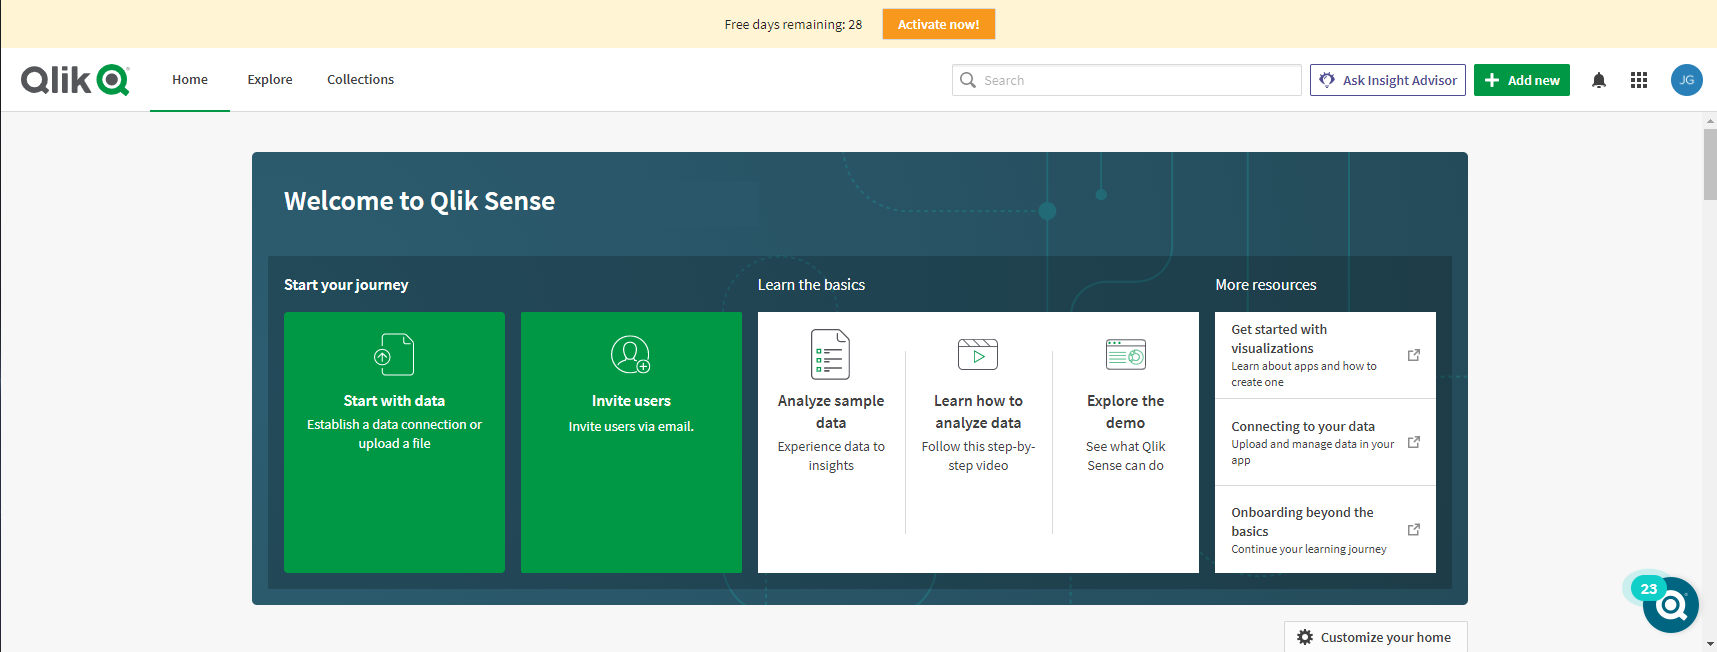
\includegraphics[width=14cm]{./images/1} 
	\end{center}
	\begin{center}
		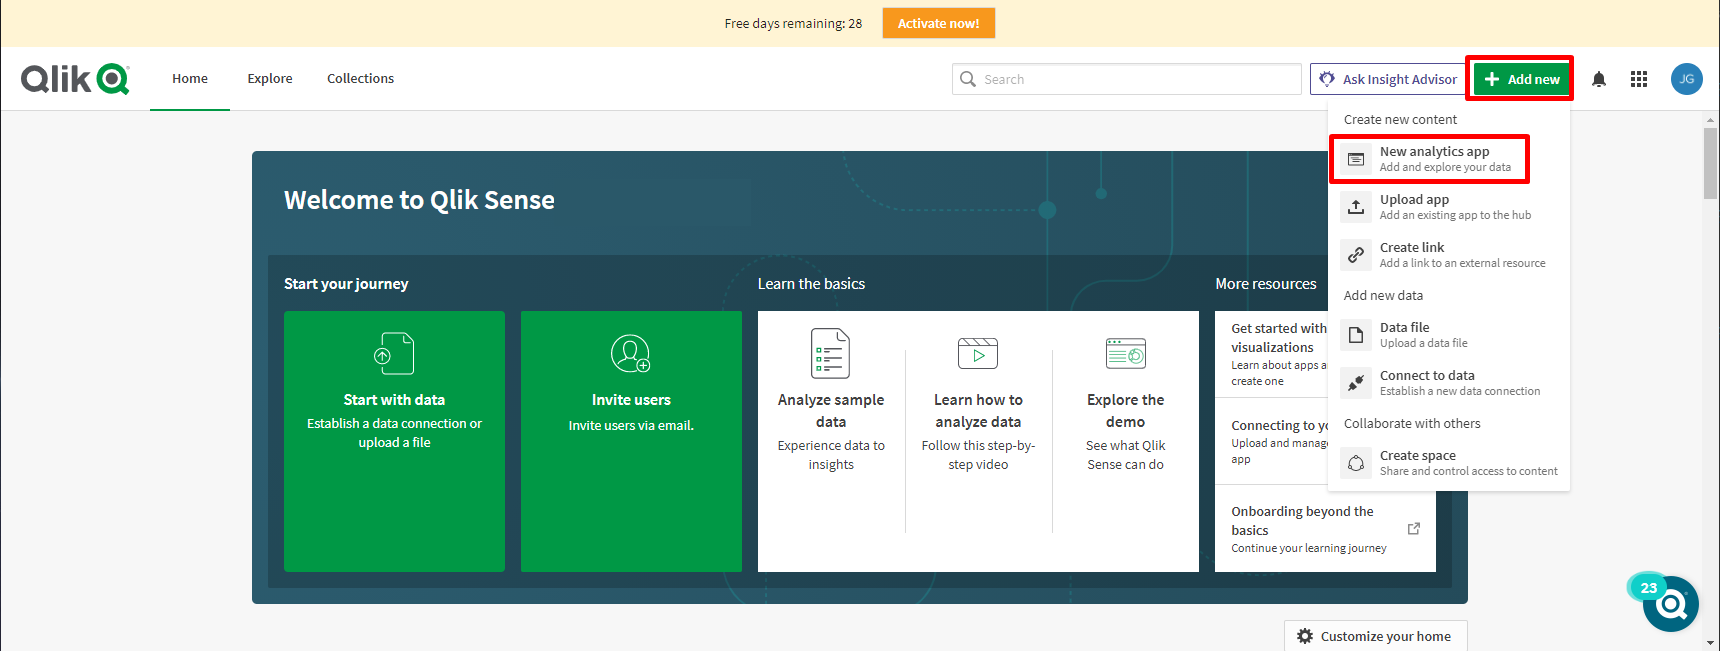
\includegraphics[width=14cm]{./images/2} 
	\end{center}
	 \begin{center}
		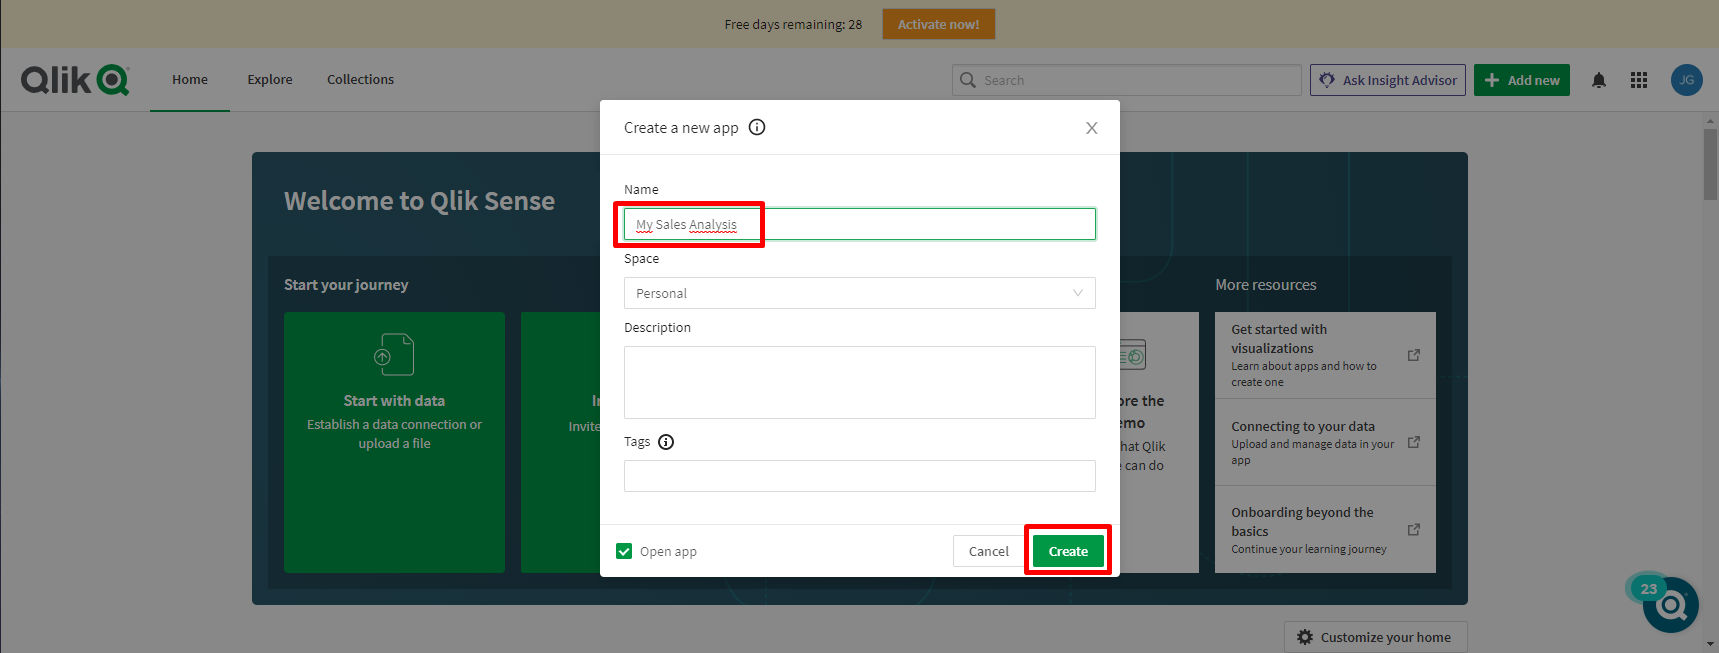
\includegraphics[width=14cm]{./images/2.1} 
	\end{center}
	\begin{center}
		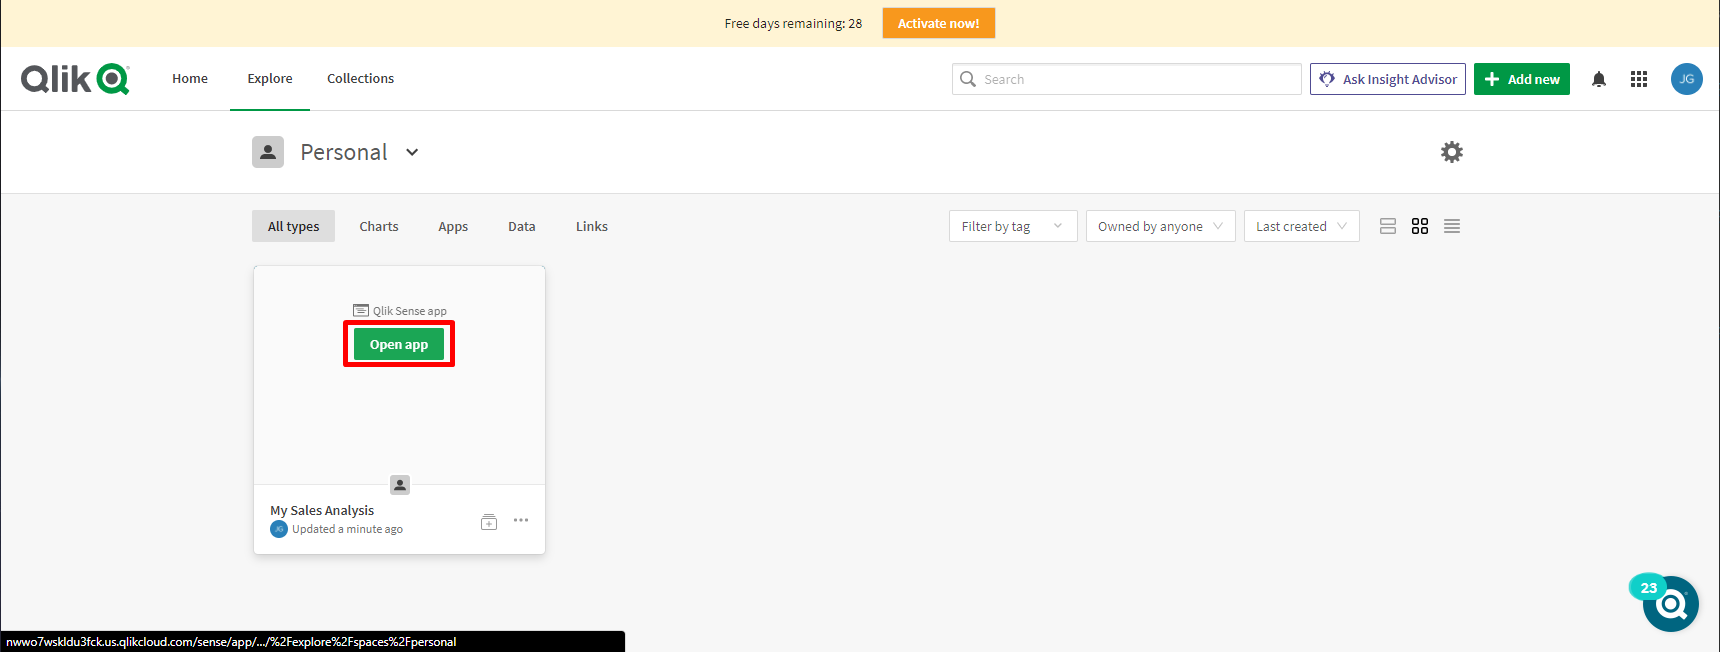
\includegraphics[width=14cm]{./images/2.2} 
	\end{center}

\section{Cargar datos}

\textbf{2.1.Agregar datos de archivos y otras fuentes para agregar los datos del Excel a la aplicación}

    \begin{center}
		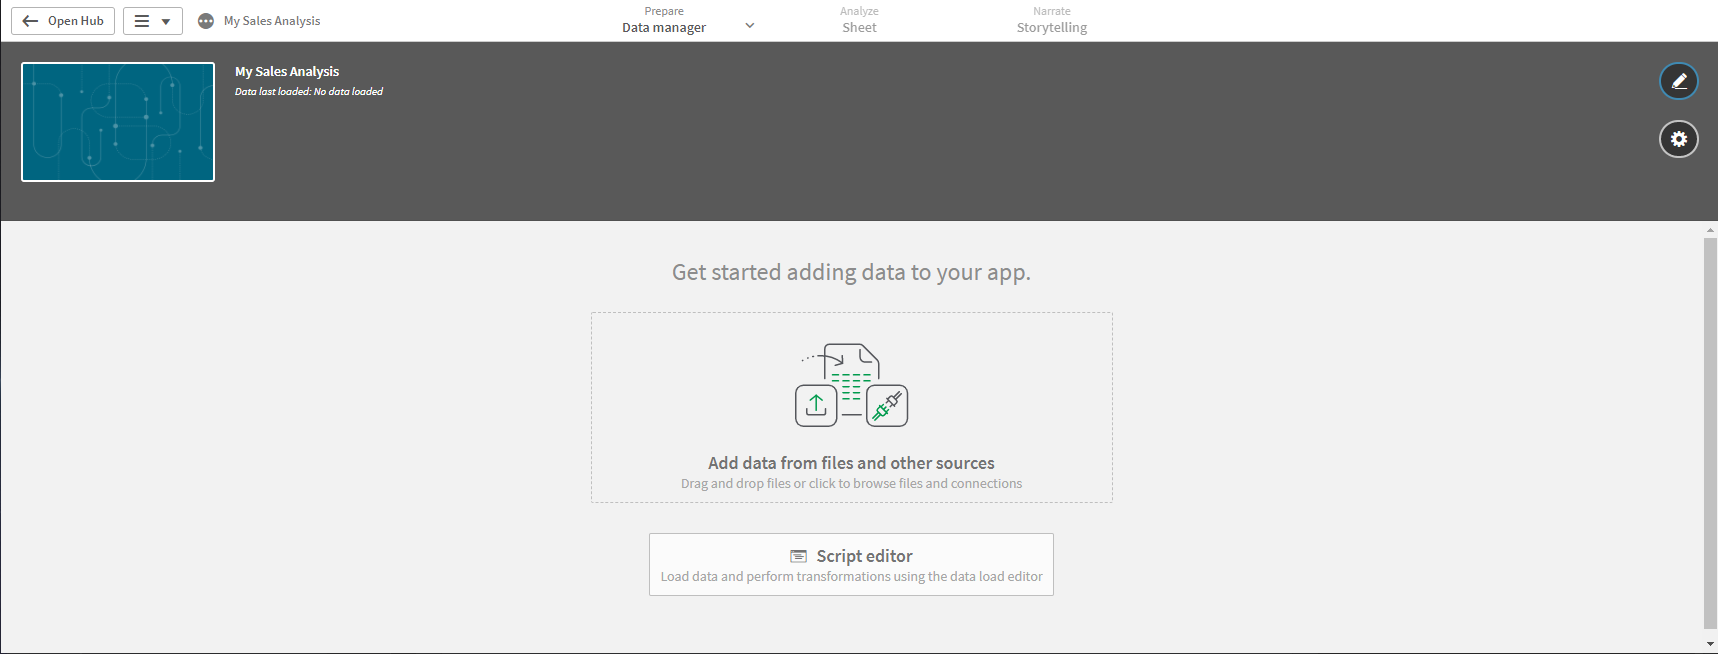
\includegraphics[width=14cm]{./images/3} 
	\end{center}
	
	
\newpage
\textbf{2.2.  Cargue todos los campos de la hoja de cálculo, haciendo clic en el botón}

    \begin{center}
		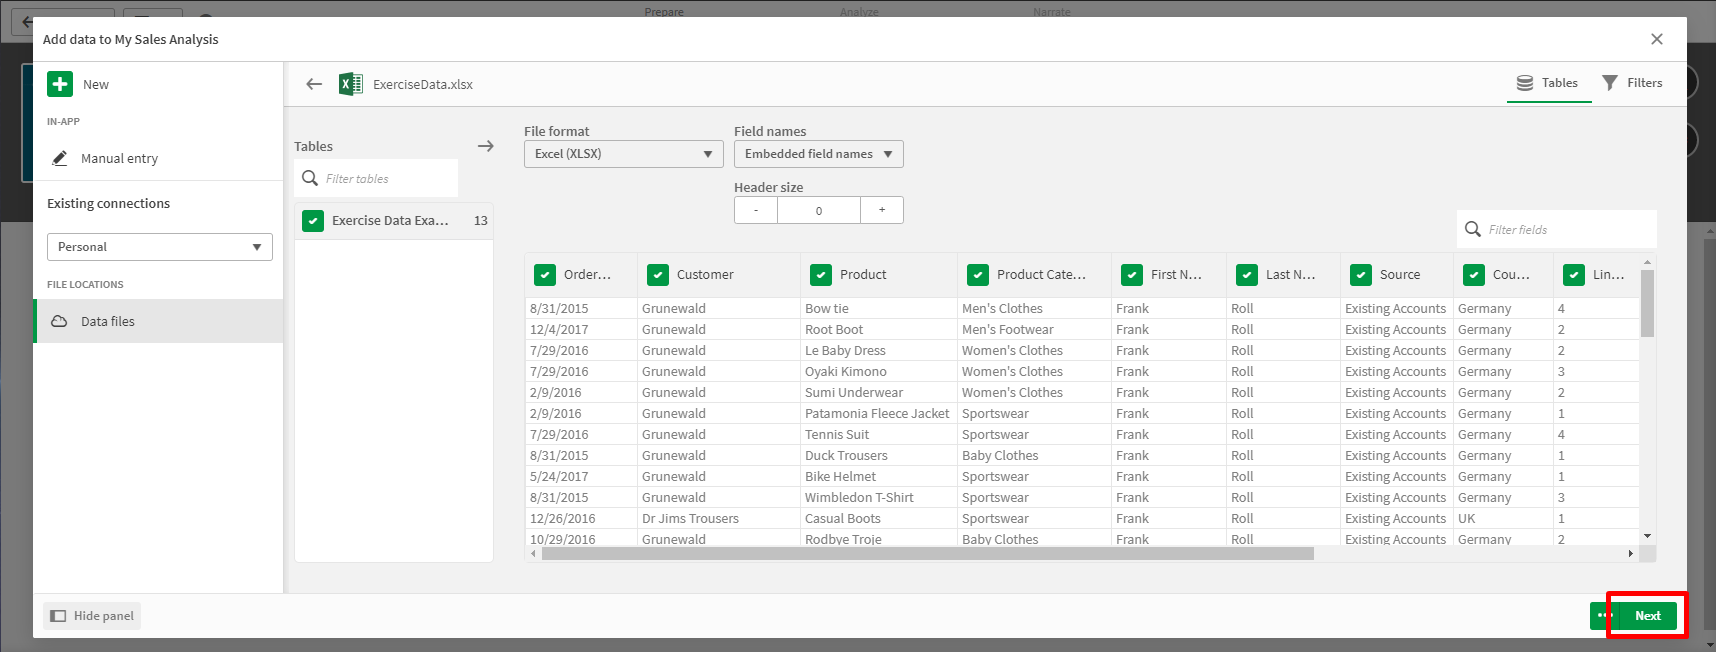
\includegraphics[width=14cm]{./images/3.1} 
	\end{center}
	
\section{Revisar datos}

\textbf{3.1.Utilice el menú de acceso rápido para navegar a la 
vista del Administrador de datos y obtener más información sobre esta tabla.}

    \begin{center}
		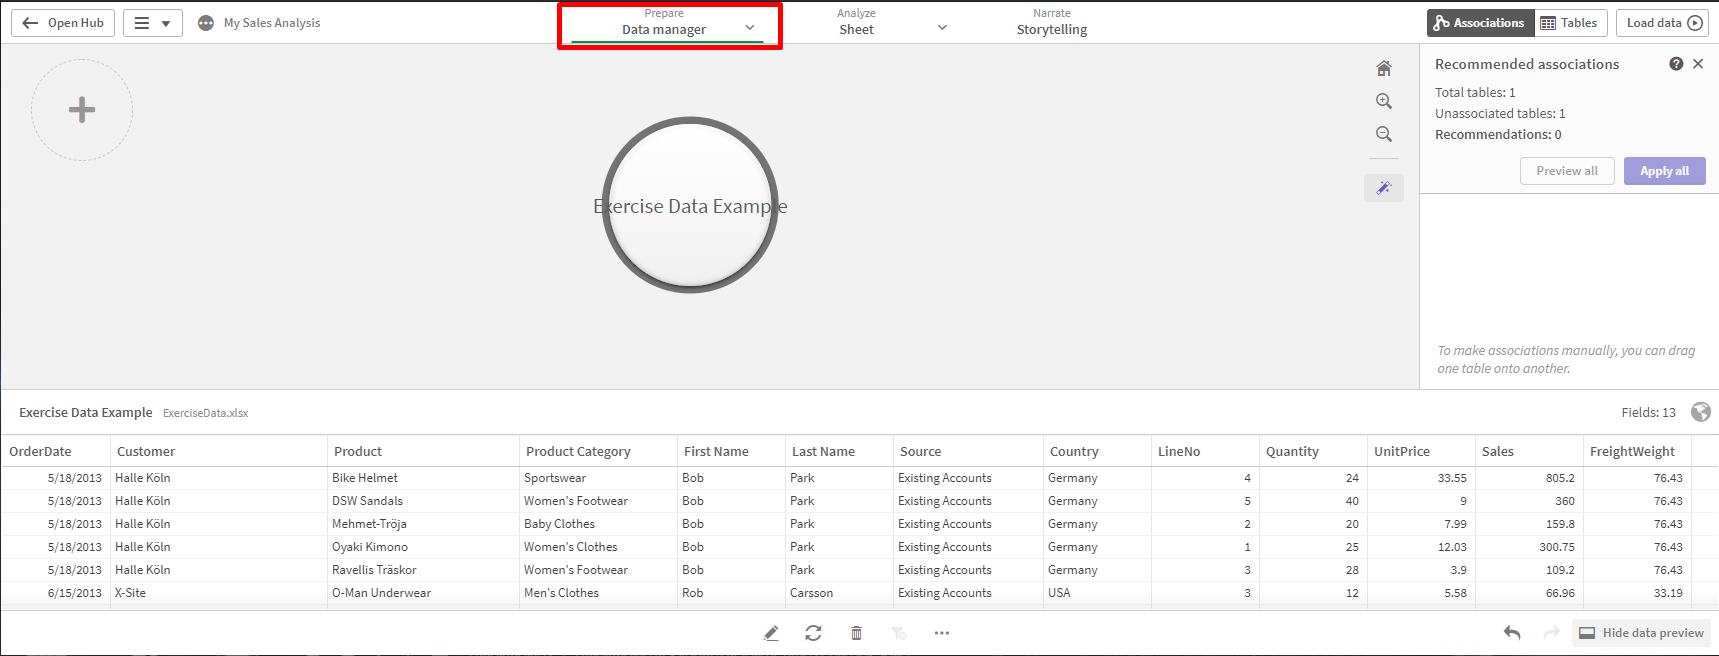
\includegraphics[width=14cm]{./images/4} 
	\end{center}
	
	\newpage
\textbf{3.2. Abra la vista del editor de tablas del 
administrador de datos haciendo clic en el ícono de lapiz
 en la parte inferior de la vista.}

    \begin{center}
		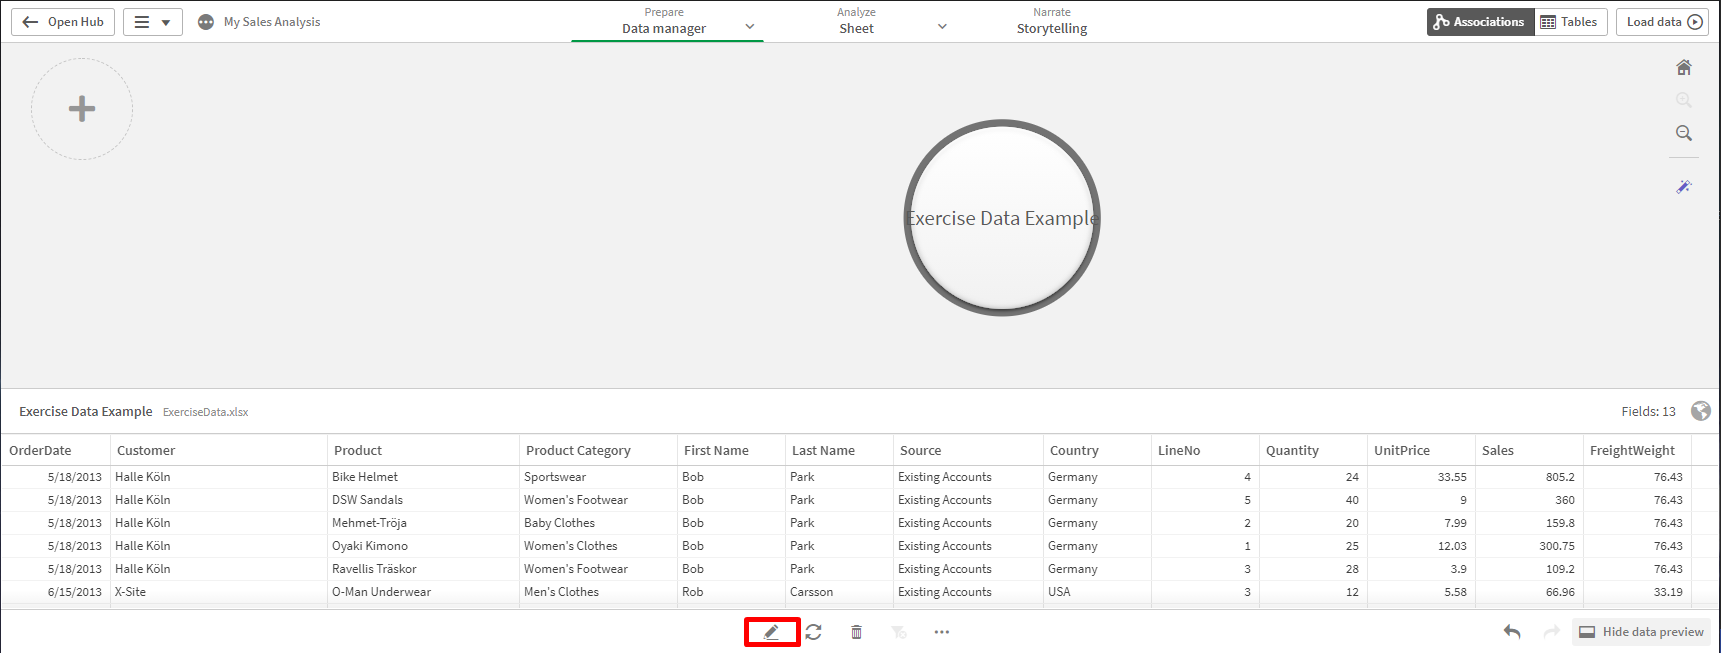
\includegraphics[width=14cm]{./images/5} 
	\end{center}

\textbf{3.3. ¿Cuántos valores de 
\textit{\textbf{Country}} distintos están presentes en esta tabla?}

    \begin{center}
		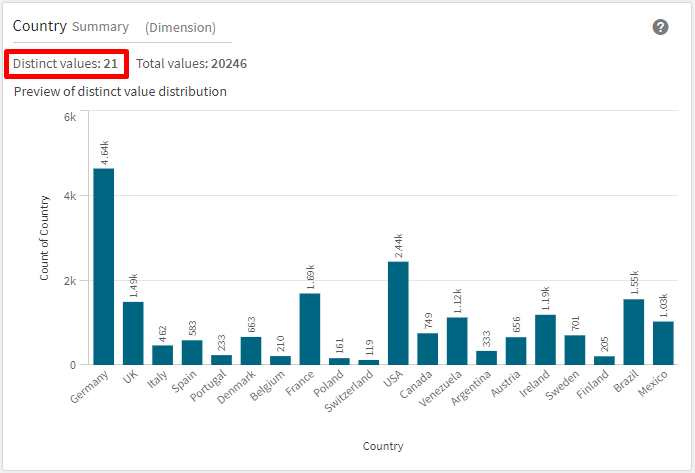
\includegraphics[width=14cm]{./images/6.1} 
	\end{center}
	\newpage
\textbf{3.4. ¿Cuántos valores
 distintos hay para la \textit{\textbf{Product Category}}}

    \begin{center}
		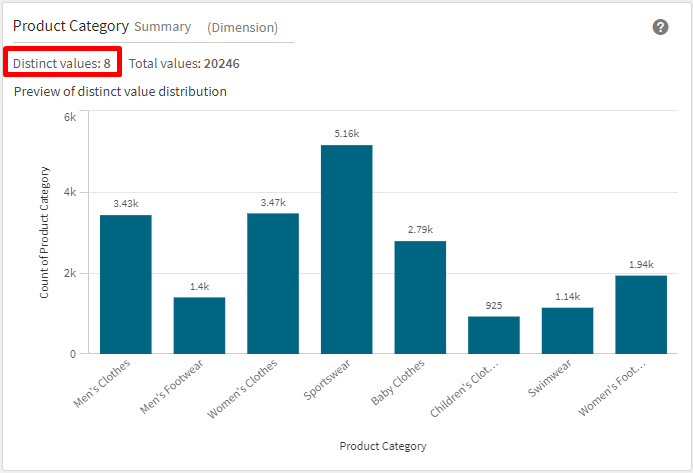
\includegraphics[width=14cm]{./images/6.2} 
	\end{center}
	\newpage
\textbf{3.5. ¿Cuántos valores distintos
 hay para el campo \textit{\textbf{Product}}}

    \begin{center}
		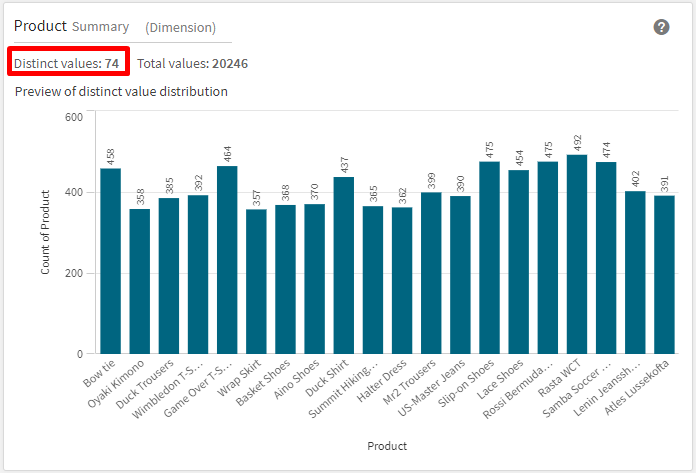
\includegraphics[width=14cm]{./images/6.3} 
	\end{center}
	
	\newpage
\textbf{3.6. ¿Cuántos valores 
distintos hay para el campo \textit{\textbf{Source}}?}

    \begin{center}
		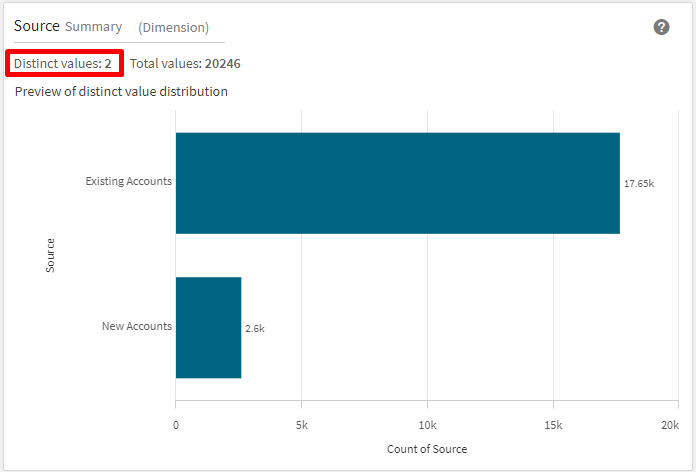
\includegraphics[width=14cm]{./images/6.4} 
	\end{center}
	
	\newpage
\textbf{3.7.¿Cuáles son esos dos valores del campo \textit{\textbf{Source}}?}

    \begin{center}
		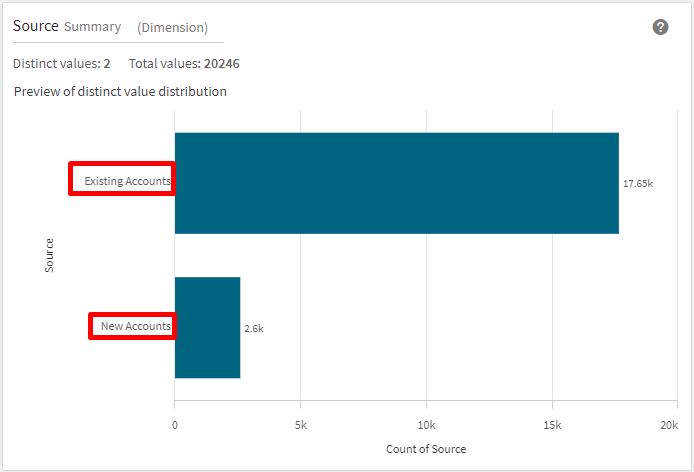
\includegraphics[width=14cm]{./images/6.5} 
	\end{center}



\section{Desarrolle una hoja con el ‘Insight advisor’}

\textbf{4.1. Use el submenú de navegación de acceso
 rápido en \textit{Analize} $>$ \textbf{Sheet} para seleccionar \textbf{Insights}..}

    \begin{center}
		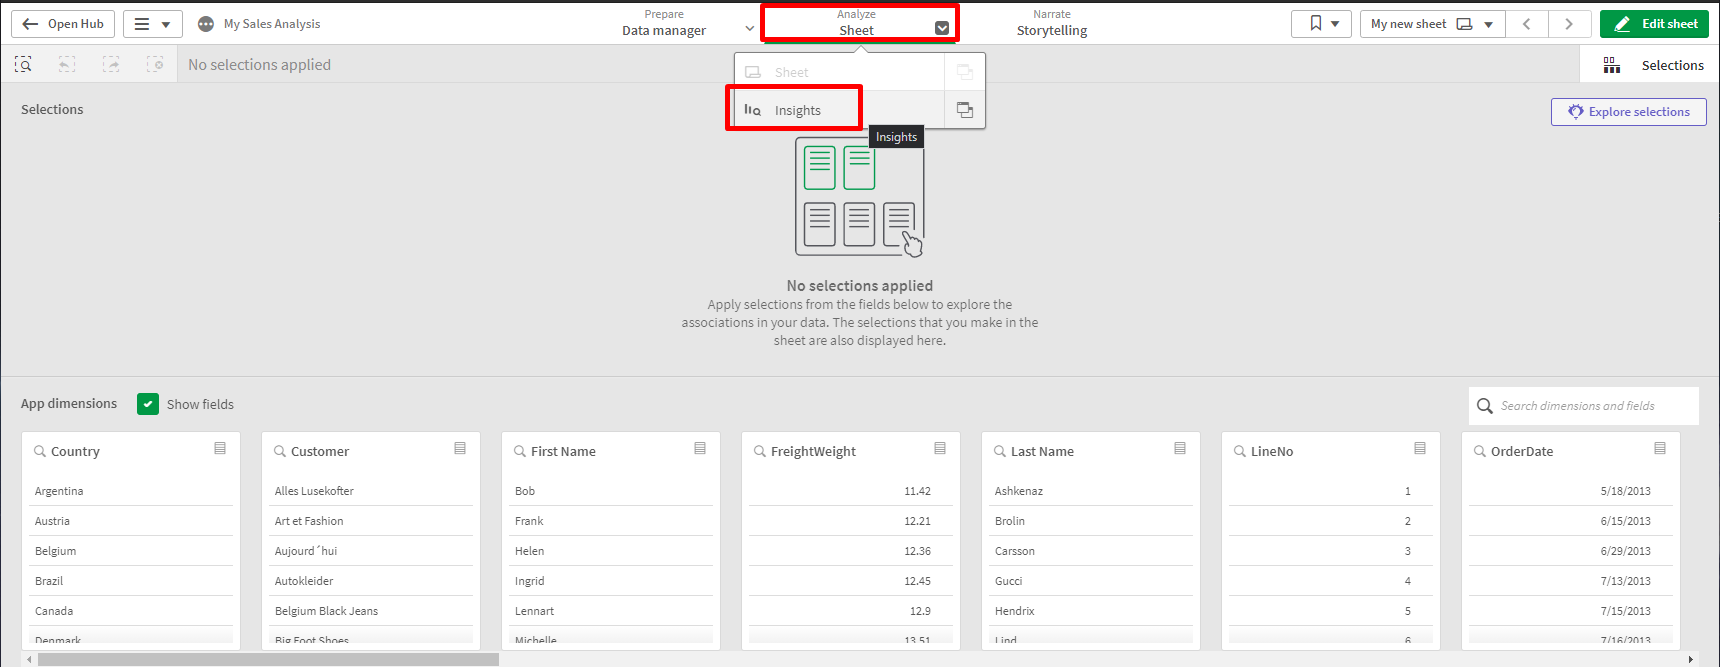
\includegraphics[width=14cm]{./images/7} 
	\end{center}

\textbf{4.2. Haga clic en el botón
 para \textbf{Generar insights}, basado en todo el modelo de datos.}

    \begin{center}
		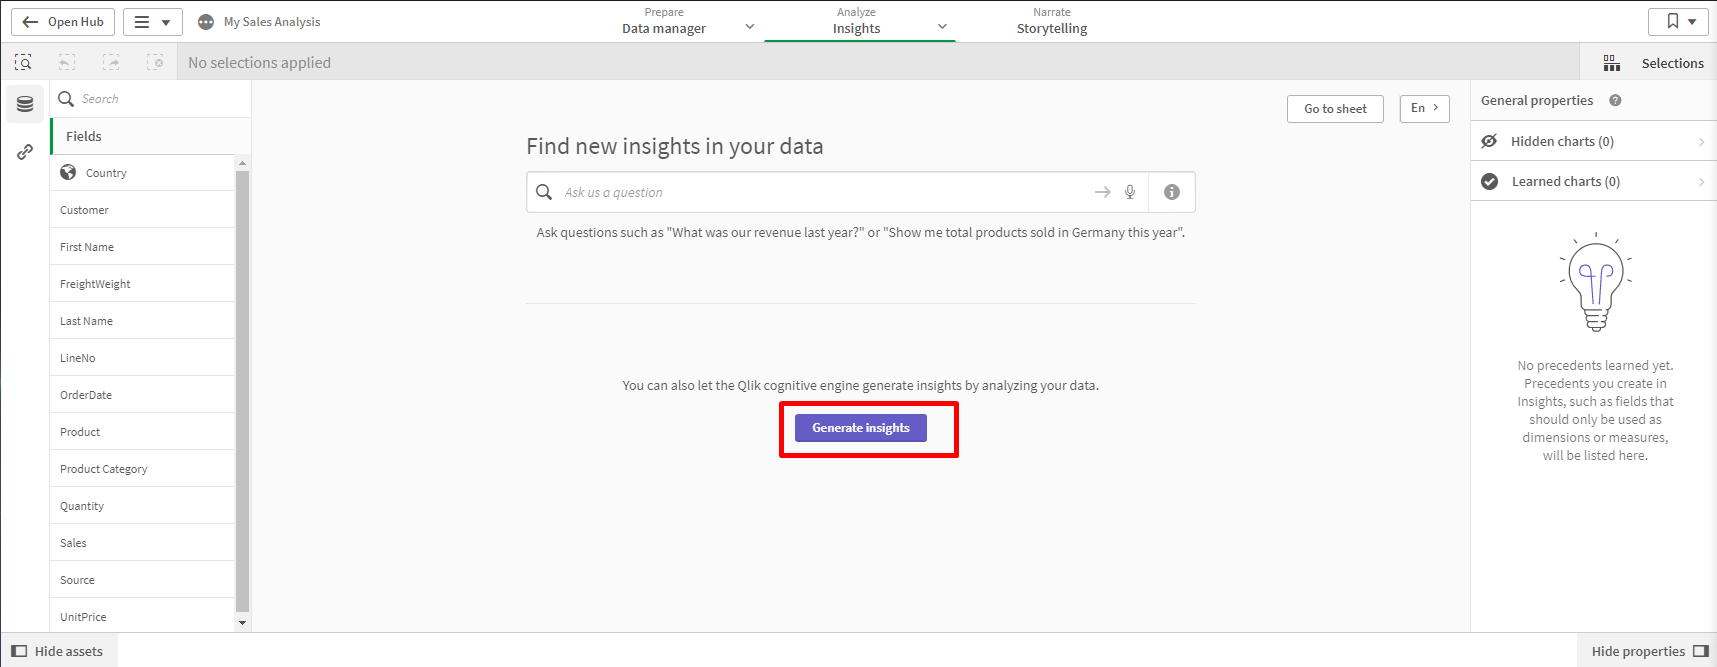
\includegraphics[width=14cm]{./images/8} 
	\end{center}
	
\textbf{4.3. Busque el mapa en la lista de gráficos
 propuestos y seleccione \textbf{Add to sheet} $>$ \textit{My new sheet}.}

    \begin{center}
		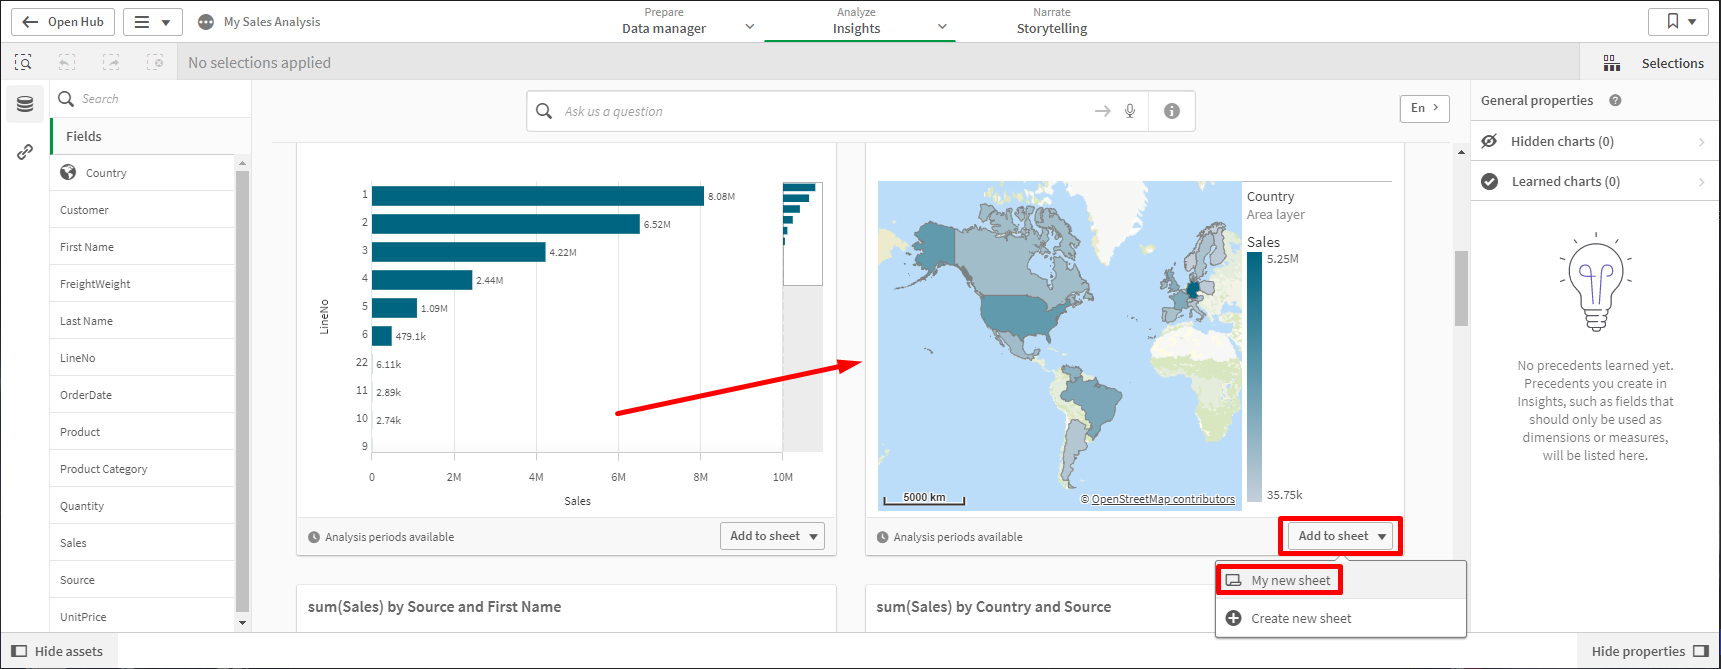
\includegraphics[width=14cm]{./images/9} 
	\end{center}
\newpage
\textbf{4.4. Utilice el panel de la izquierda
 para seleccionar (casillas marcadas) los campos:
 \textit{Product} y \textit{UnitPrice}.}

    \begin{center}
		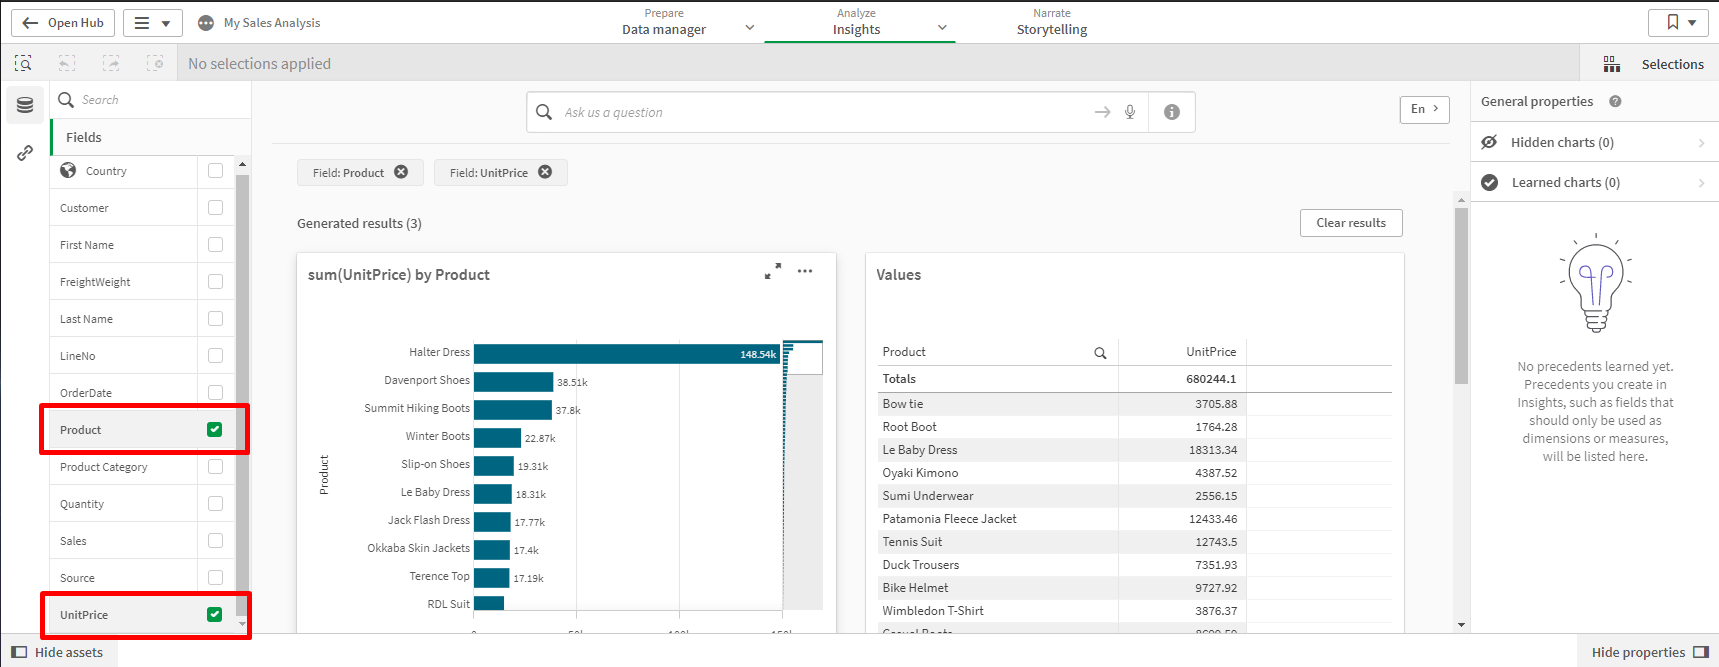
\includegraphics[width=14cm]{./images/10} 
	\end{center}
	
\textbf{4.5. Busque el gráfico de barras
 titulado: \textit{sum(UnitPrice) by Product} y sleccione 
\textbf{Add to sheet} $>$  \textit{My new sheet}.}

    \begin{center}
		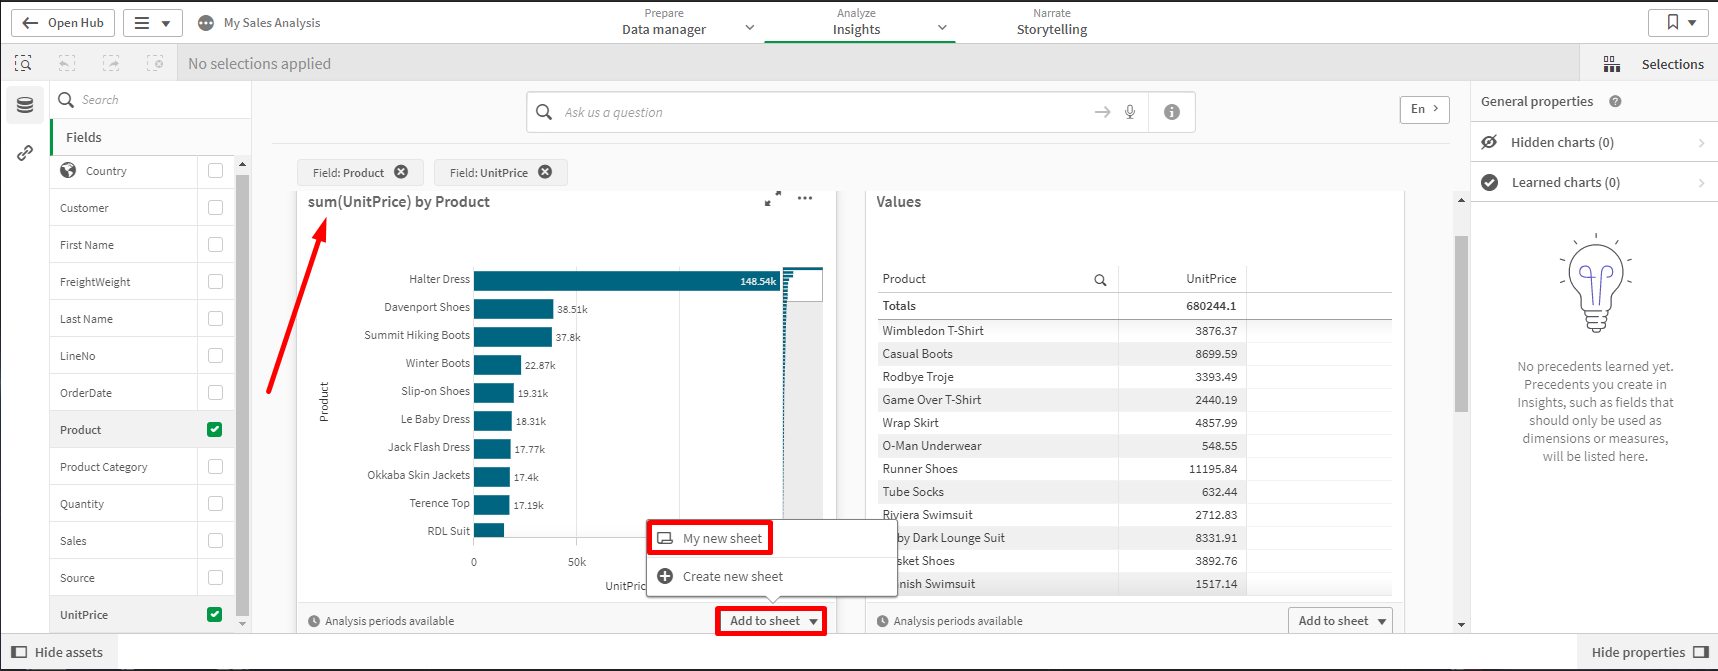
\includegraphics[width=14cm]{./images/10.1} 
	\end{center}
\newpage
\textbf{4.6. Podemos limpiar los 
filtros haciendo clic en la \textit{\textbf{'x'}}.}

    \begin{center}
		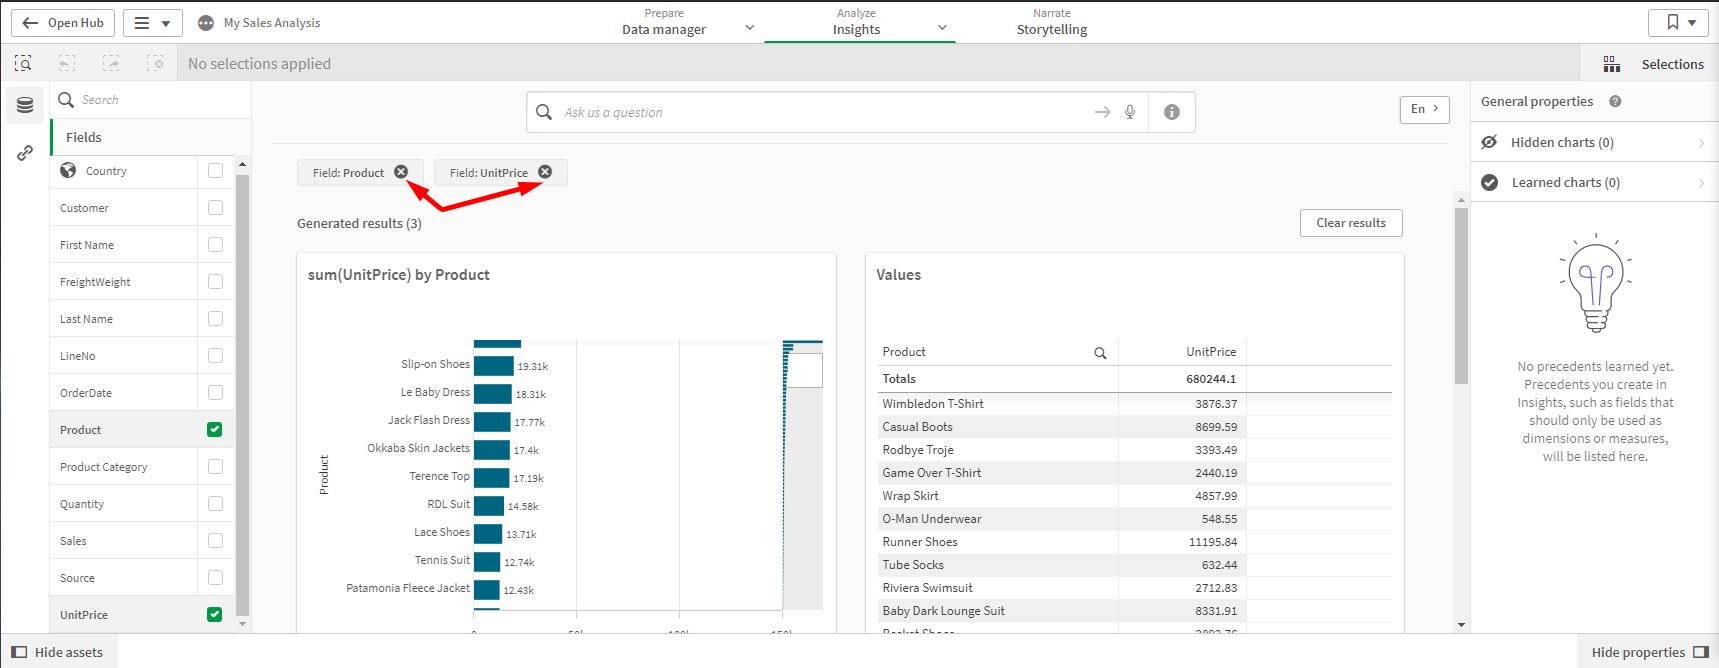
\includegraphics[width=14cm]{./images/10.2} 
	\end{center}
	
\textbf{4.7. Escriba lo siguiente en el
 campo \textit{‘Ask us a question’}: 
\textbf{Which country has highest quantity?} (y enviar pregunta).}

    \begin{center}
		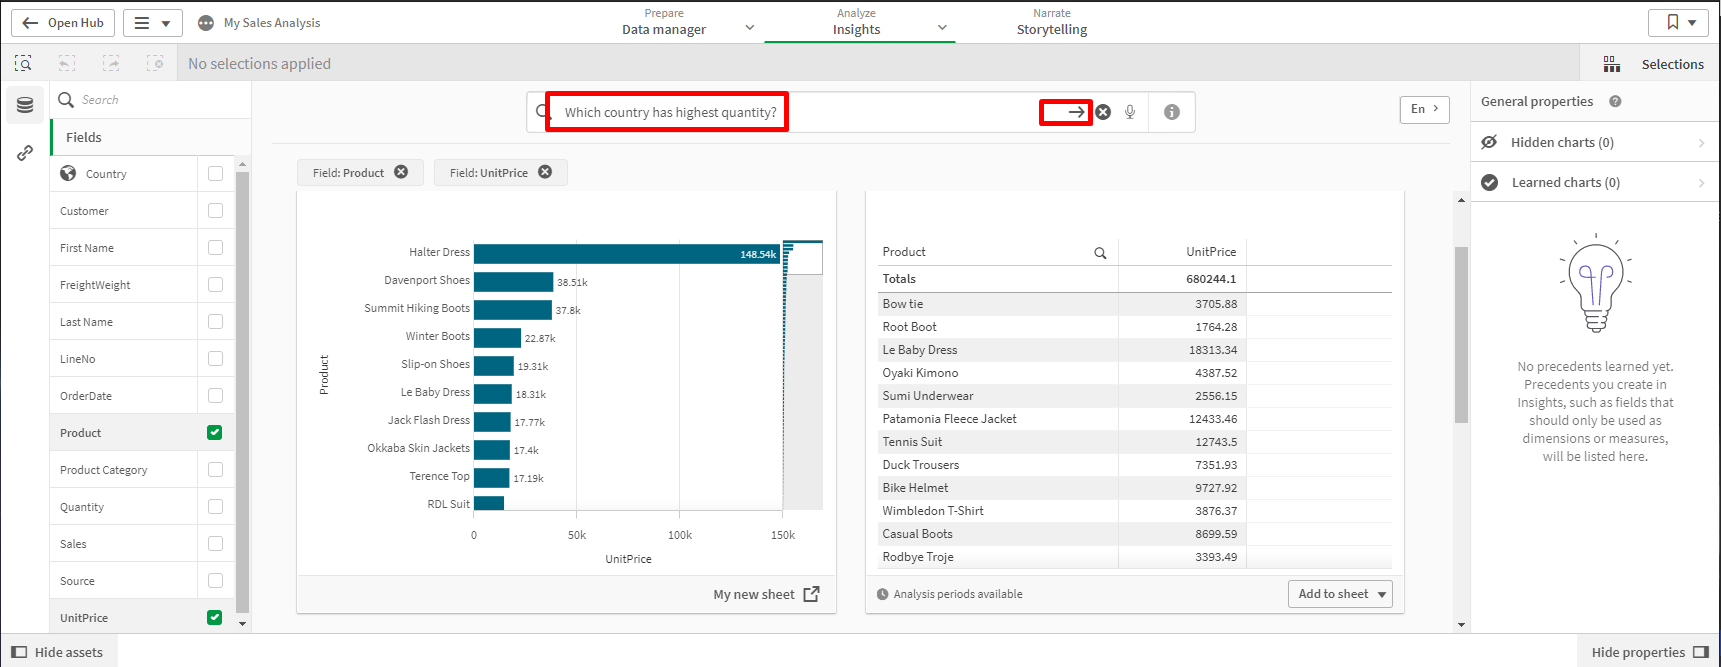
\includegraphics[width=14cm]{./images/11} 
	\end{center}
\newpage
\textbf{4.8. Busque el gráfico de barras
 titulado: \textit{sum(Quantity) by Country} y seleccione 
\textbf{Add to sheet} $>$ \textbf{My new sheet}.}

    \begin{center}
		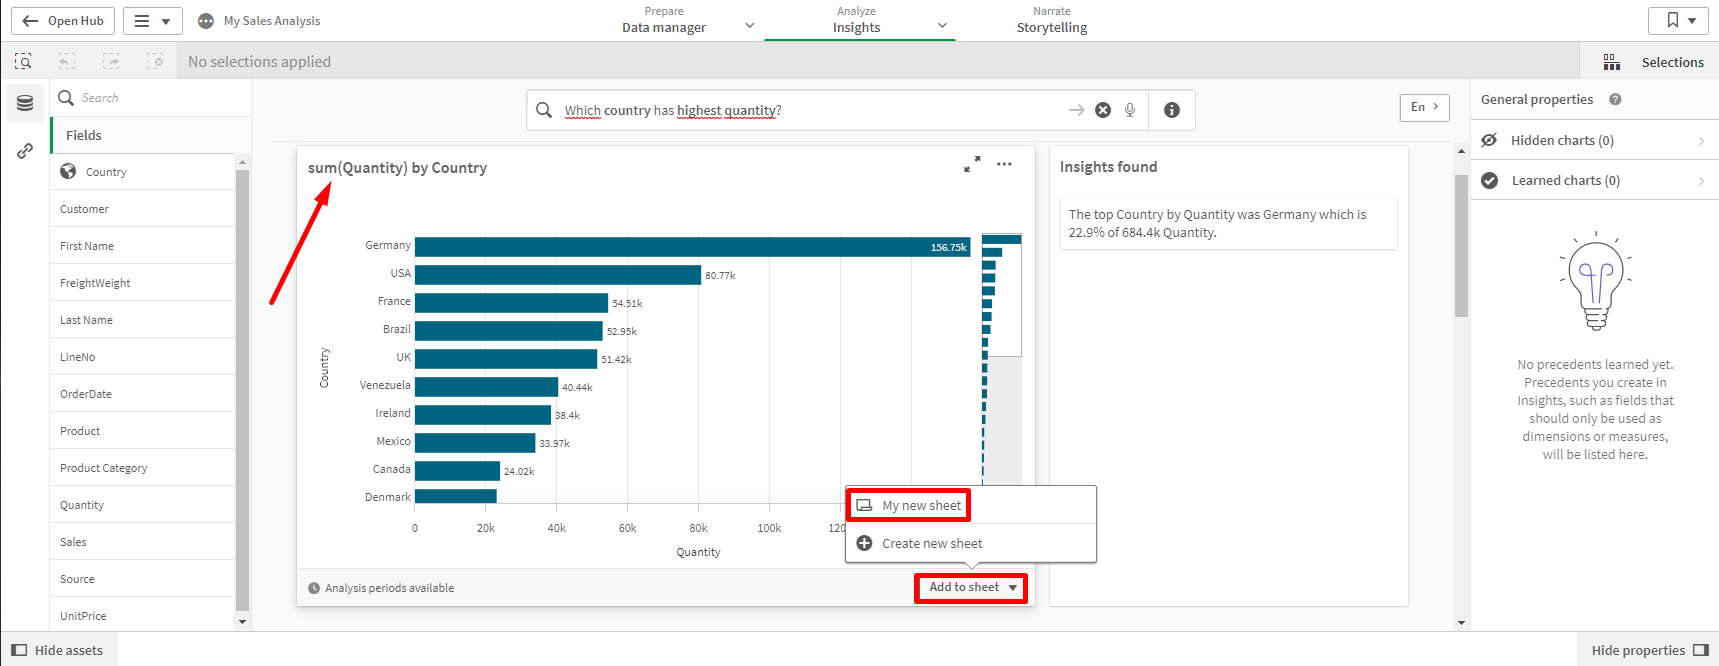
\includegraphics[width=14cm]{./images/11.1} 
	\end{center}
	
\textbf{4.9. Utilice el submenú de navegación 
de acceso rápido en \textit{Analyze} $>$ \textbf{Insights}
 para seleccionar \textbf{Sheet}.}

    \begin{center}
		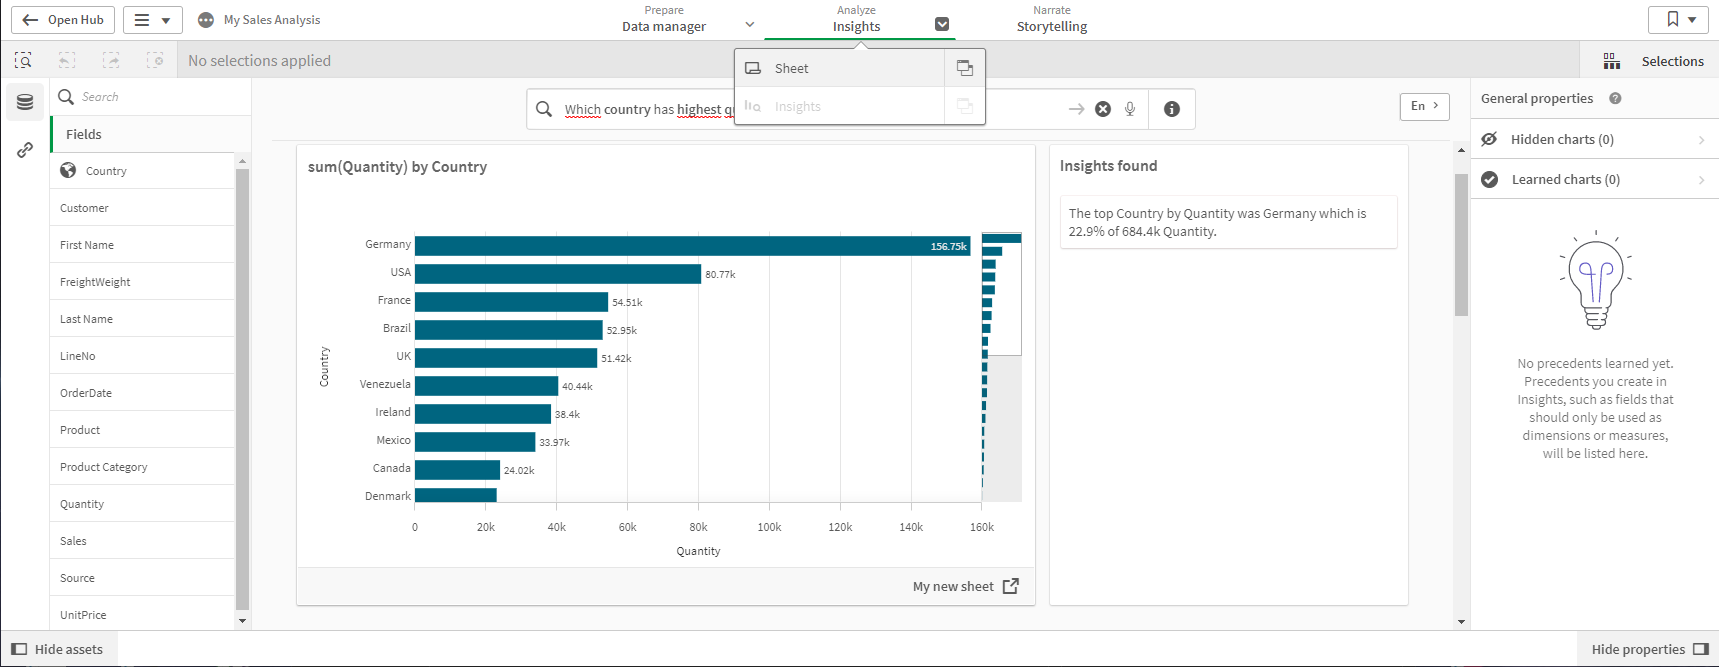
\includegraphics[width=14cm]{./images/12} 
	\end{center}

\newpage
\textbf{4.10. Evaluar la hoja que ha creado.
 Debería aparecer como ve a continuación:}

    \begin{center}
		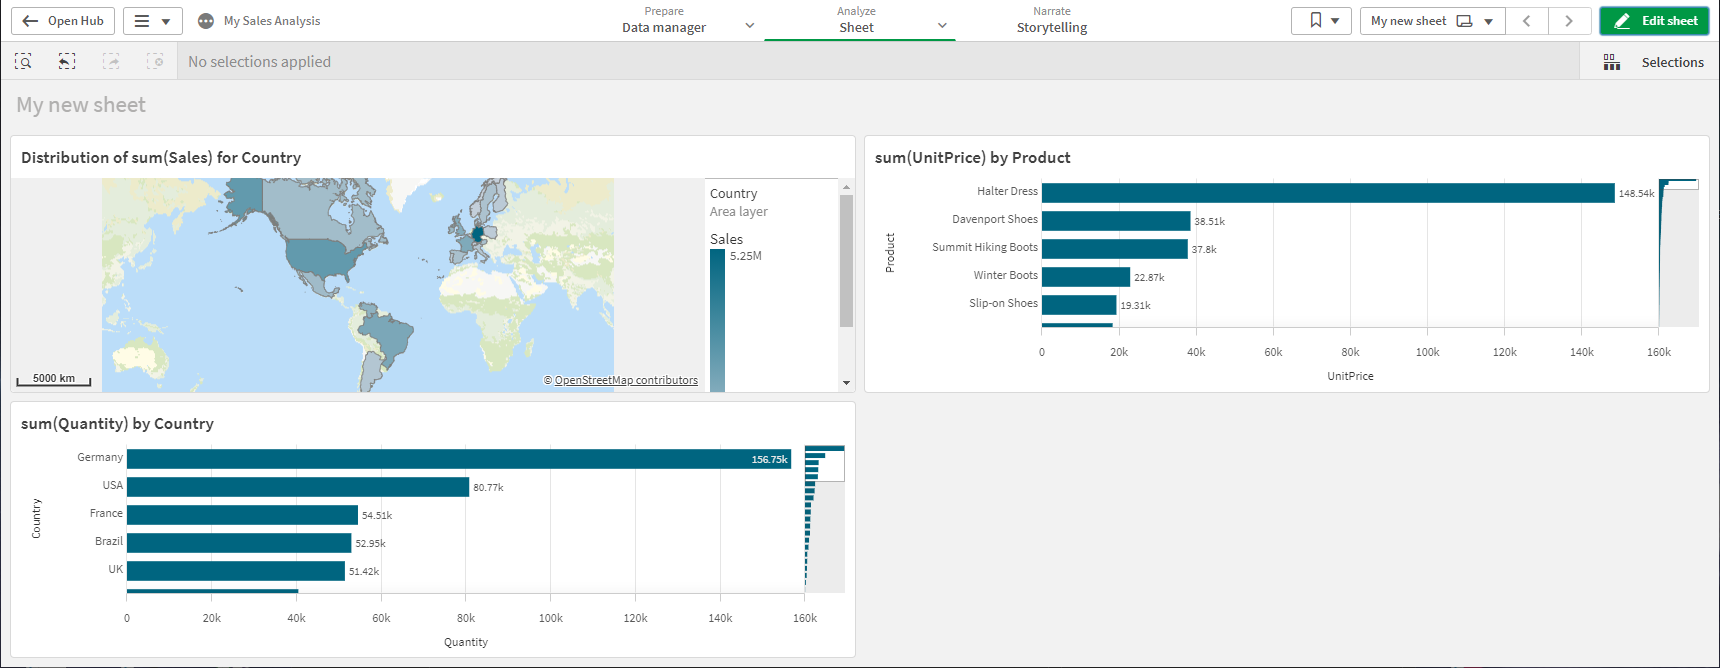
\includegraphics[width=14cm]{./images/13} 
	\end{center}
	
\textbf{4.11. Cambie la hoja al modo
 de \textbf{Edición} (el lapiz) y use el panel de 
propiedades para cambiar el título de la hoja.}

    \begin{center}
		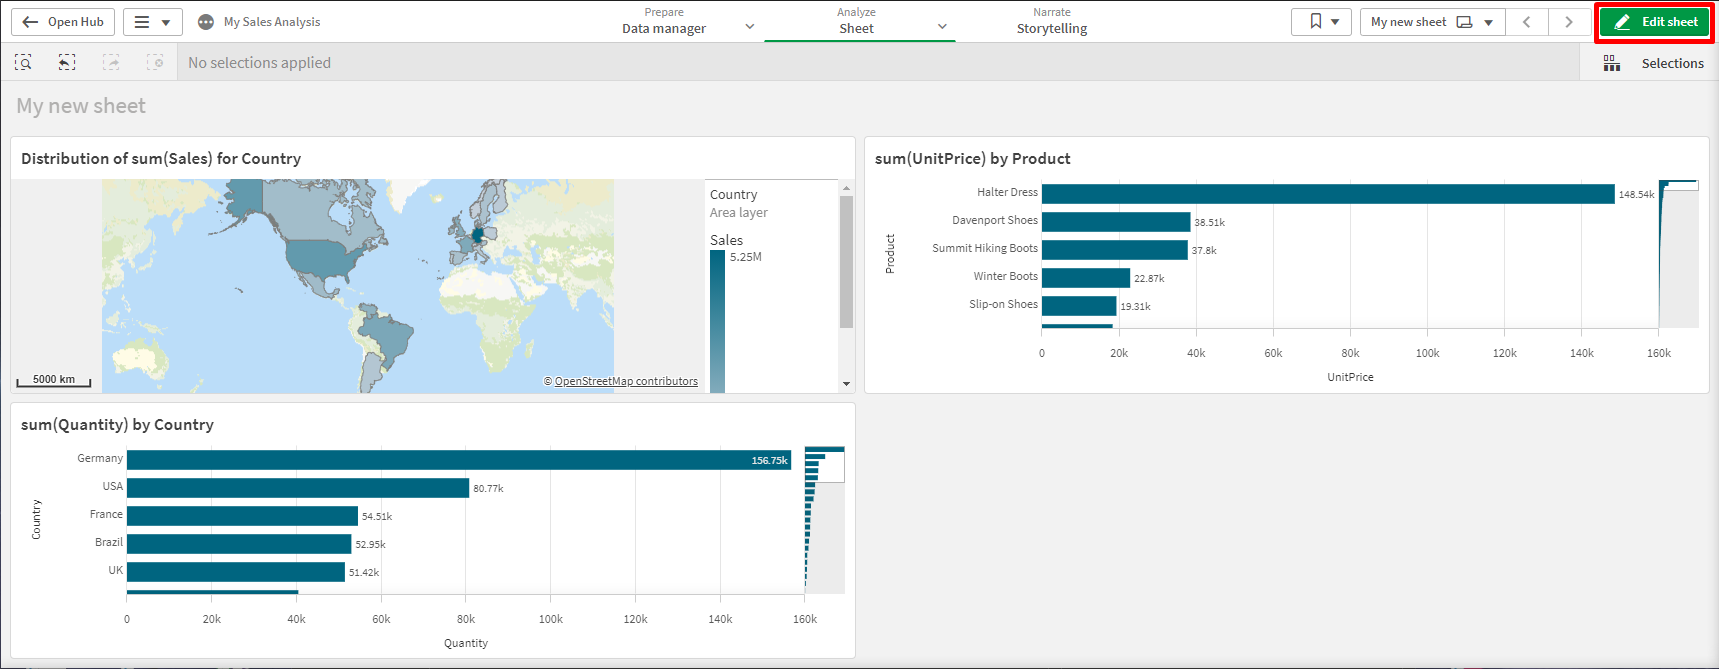
\includegraphics[width=14cm]{./images/14} 
	\end{center}
\newpage
\textbf{4.12. Cambiar el 
título de la hoja de \textit{\textbf{“My new sheet”}} a
 \textit{\textbf{“My insights”}} y para terminar la edicion 
 clic en el boton \textbf{"Done editing"}.}

    \begin{center}
		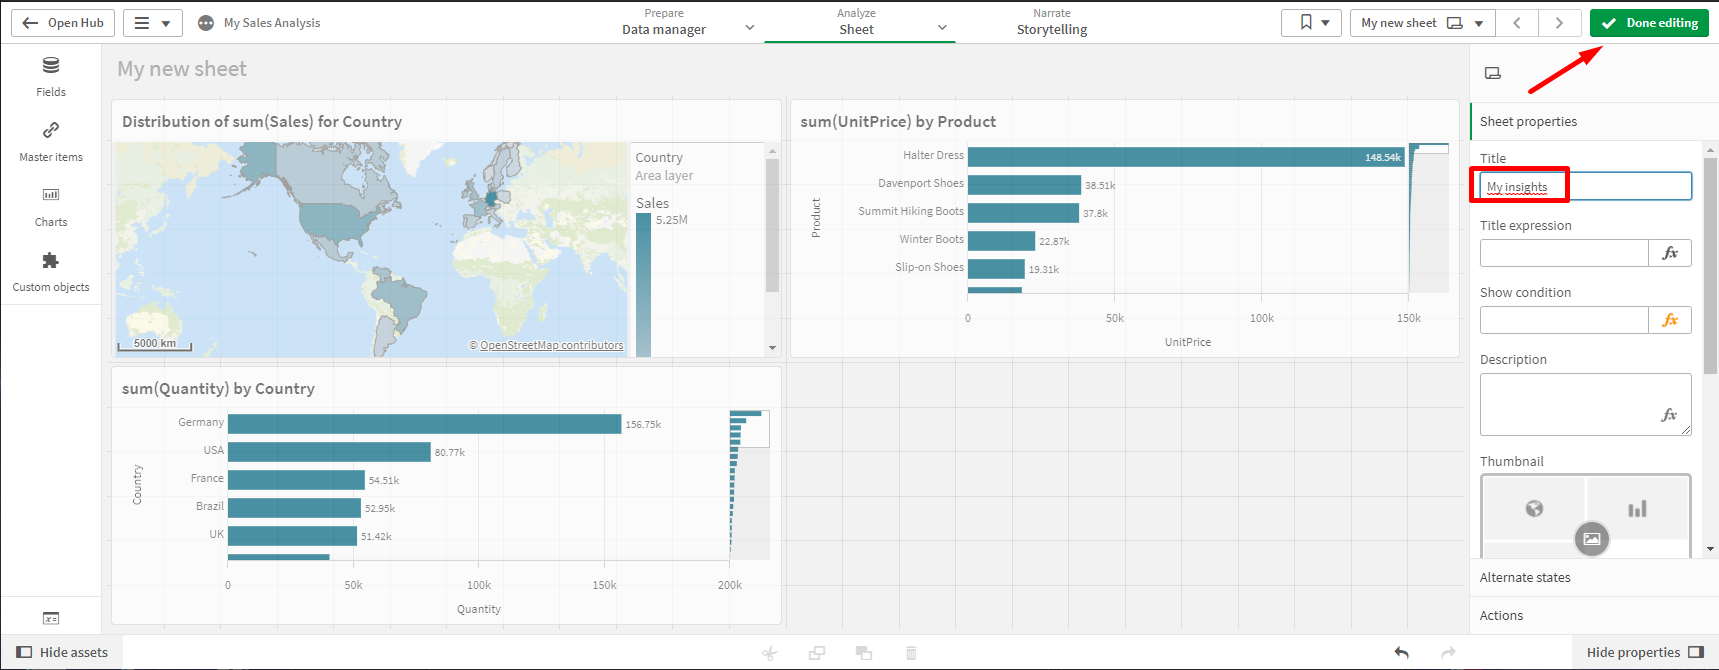
\includegraphics[width=14cm]{./images/15} 
	\end{center}
	
\newpage
\section{Desarrolle una hoja utilizando ‘Chart suggestion assistance’}

\textbf{5.1. Utilice el menú desplegable de hojas (icono de hoja) para crear una nueva hoja.}

    \begin{center}
		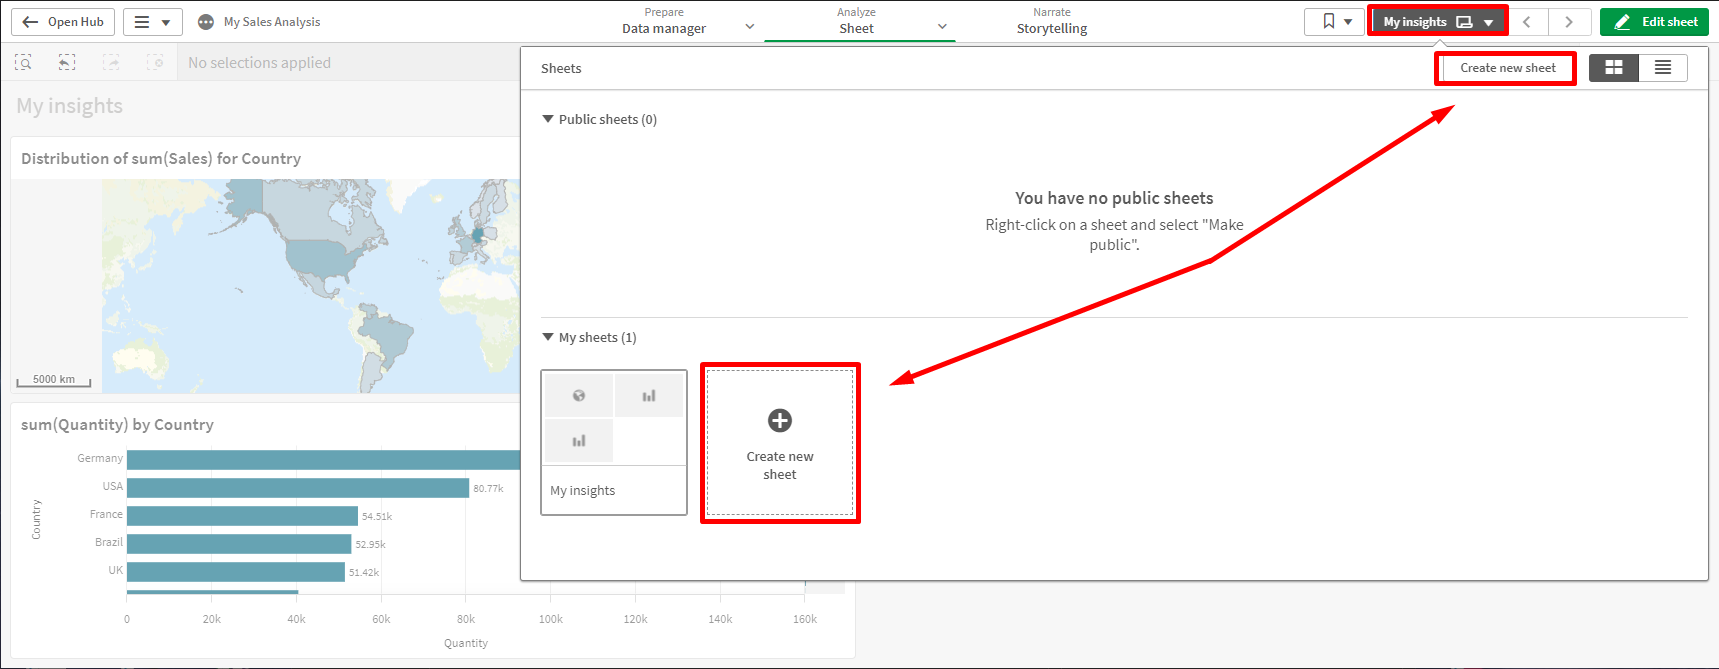
\includegraphics[width=14cm]{./images/16} 
	\end{center}
	
\textbf{5.2. Coloquele de titulo a la hoja: \textit{\textbf{“My suggestions“}}.}

    \begin{center}
		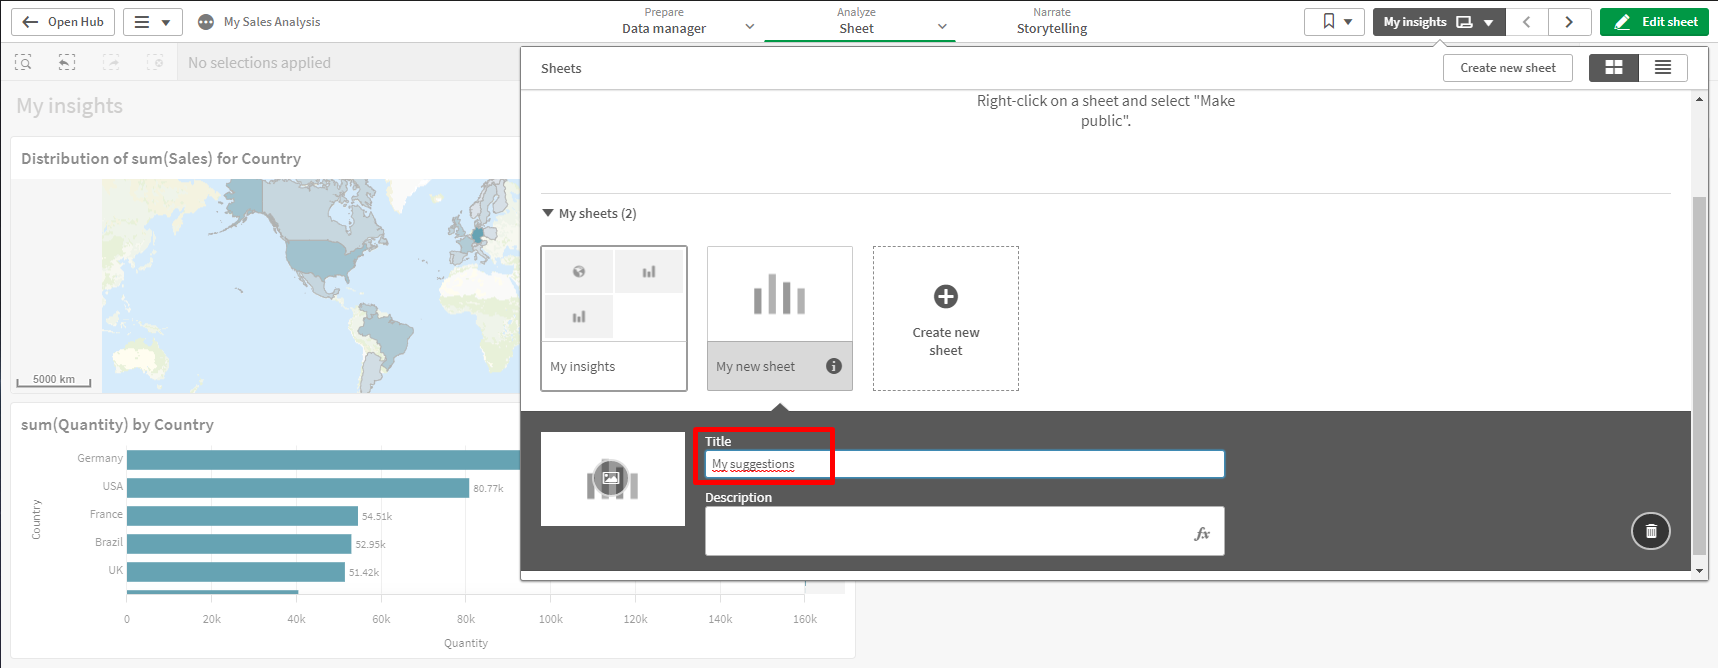
\includegraphics[width=14cm]{./images/16.1} 
	\end{center}
\newpage
\textbf{5.3. En el modo Editar hoja, use la sección Campos (icono de BD) del panel 
de activos, arrastre y suelte el campo \textit{\textbf{Sales}} en el área de visualización.}

    \begin{center}
		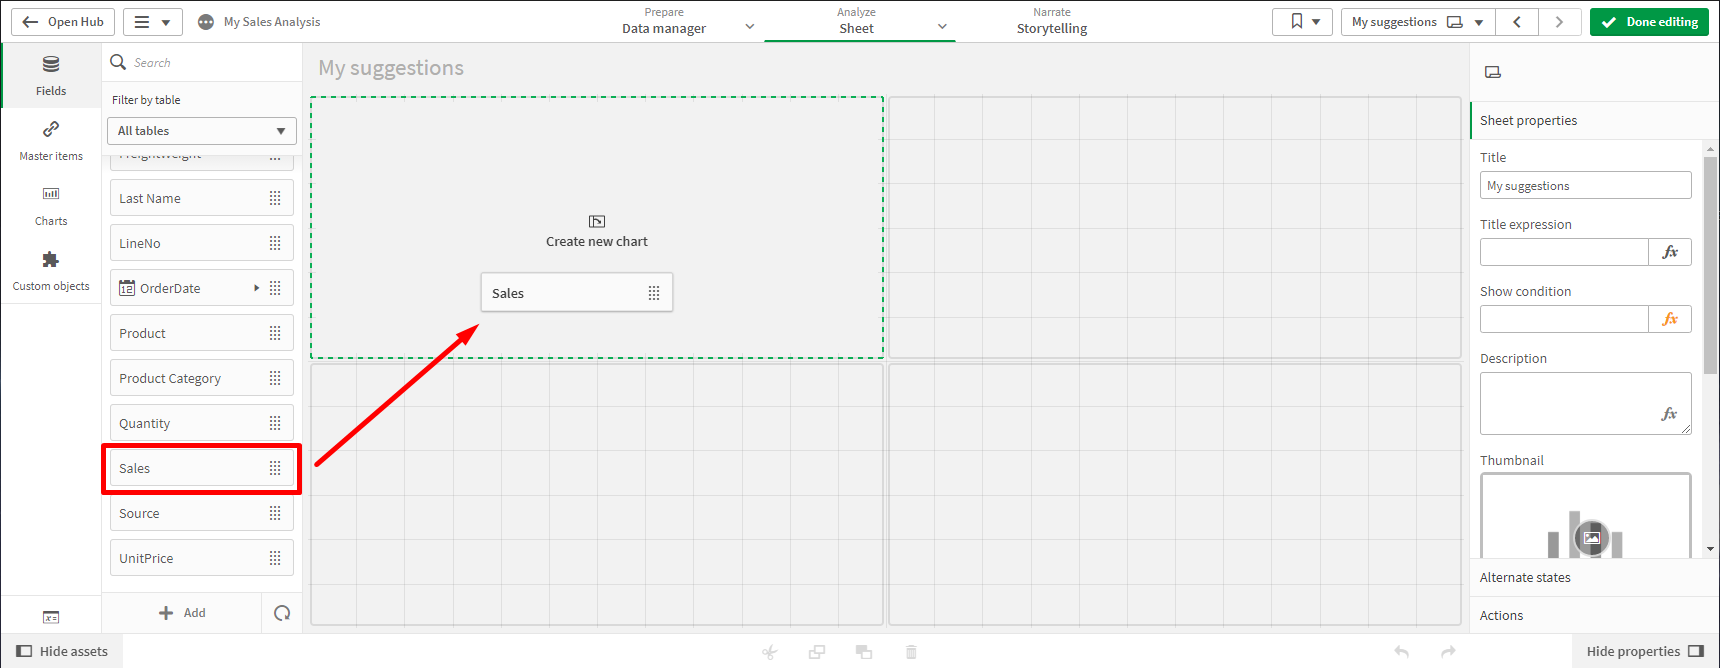
\includegraphics[width=14cm]{./images/17} 
	\end{center}

\textbf{5.4. Se obtiene un tipo de gráfico de KPI, que muestra 
la suma de los valores de ventas para todo el modelo de datos.}

    \begin{center}
		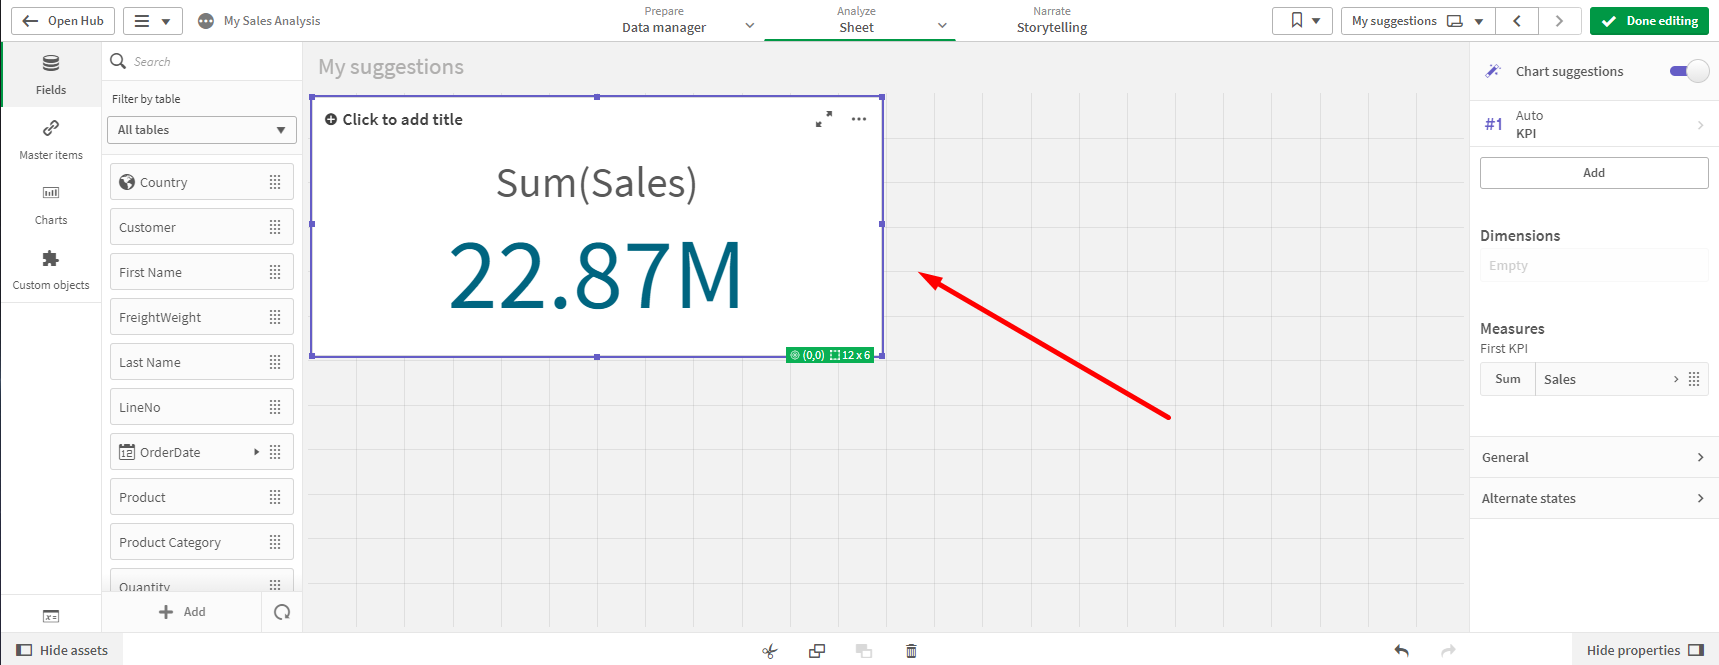
\includegraphics[width=14cm]{./images/17.1} 
	\end{center}
\newpage
\textbf{5.5. Además, el interruptor 
de \textit{\textbf{Sugerencias de Gráficos}} en la parte superior del panel de propiedades está "activado".}

    \begin{center}
		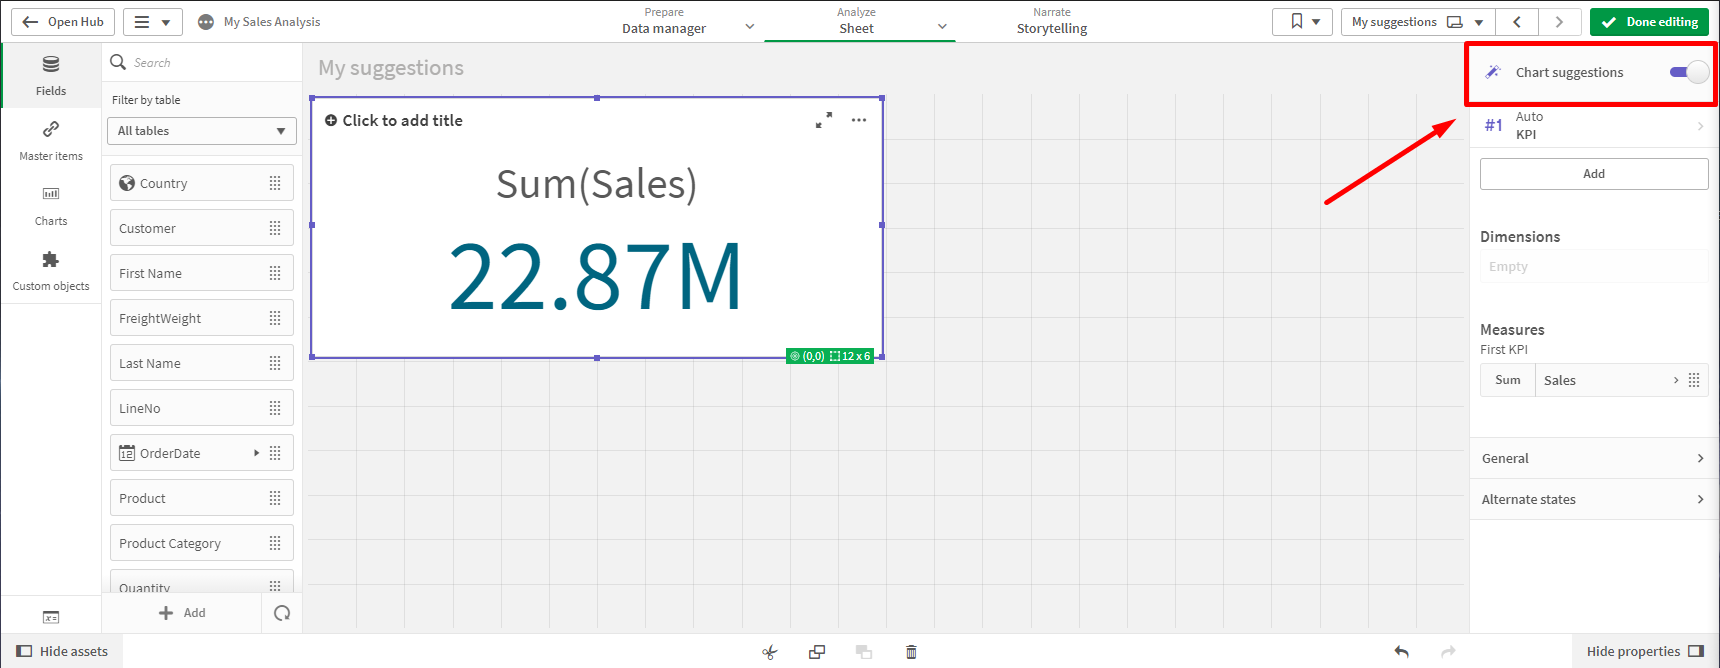
\includegraphics[width=14cm]{./images/17.2} 
	\end{center}

\textbf{5.6. Arrastre y suelte el
 campo \textit{Country} en el gráfico de KPI, asegurándose de que la imagen "fantasma" cubra todo el gráfico.}

    \begin{center}
		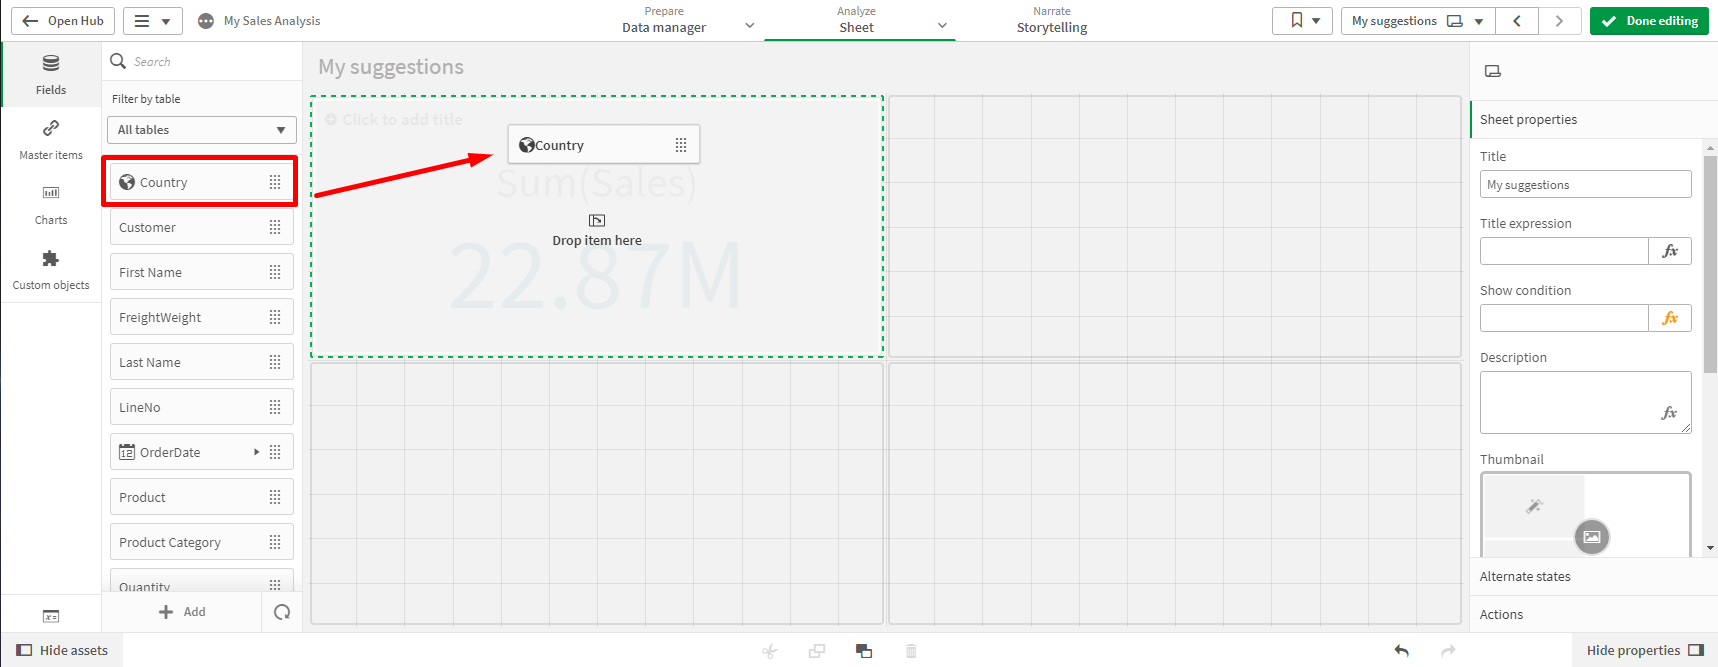
\includegraphics[width=14cm]{./images/18} 
	\end{center}
\newpage
\textbf{5.7. Se obtiene un tipo de
 gráfico de mapa y el color del mapa relaciona la suma de los valores de ventas en cada país.}

    \begin{center}
		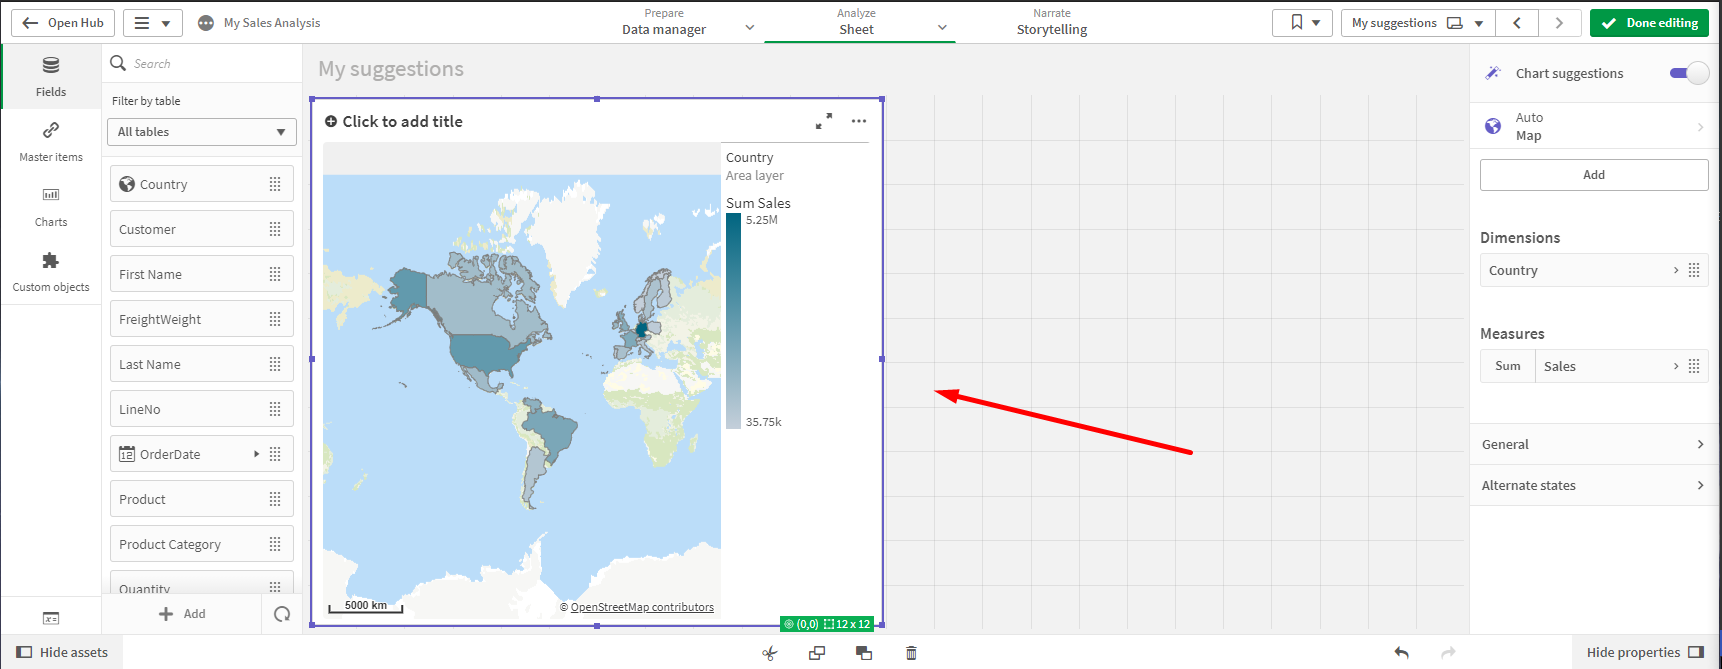
\includegraphics[width=14cm]{./images/18.1} 
	\end{center}


\newpage
\section{Desarrolle una hoja usando ‘Chart suggestion assistance’ (cont’d)}

\textbf{6.1. Expanda el campo \textit{OrderDate} en el panel de 
activos para exponer agrupaciones de fechas derivadas.}

    \begin{center}
		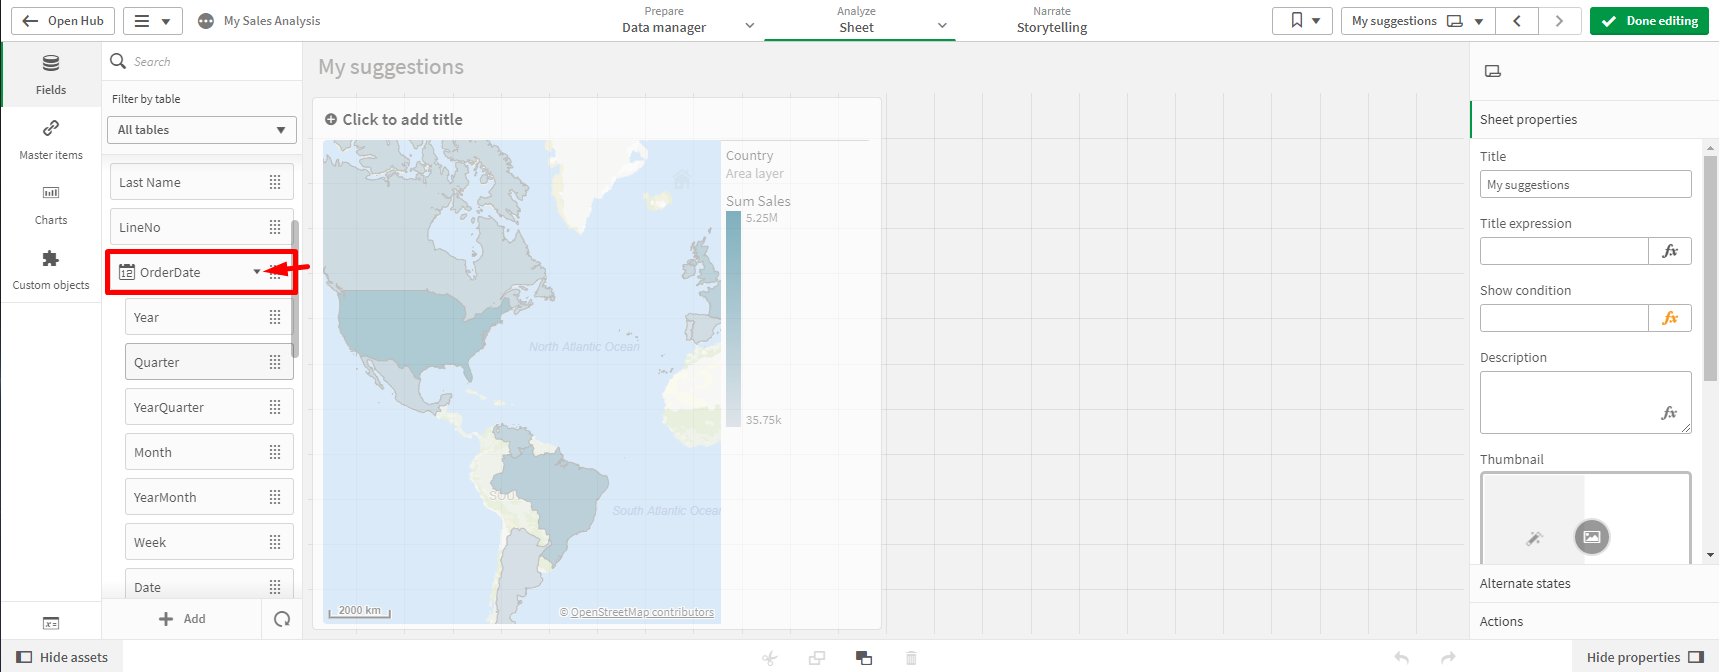
\includegraphics[width=14cm]{./images/19} 
	\end{center}


\textbf{6.2. Arrastre y suelte la agrupación \textit{YearMonth} 
en un espacio vacío en el área de visualización.}

    \begin{center}
		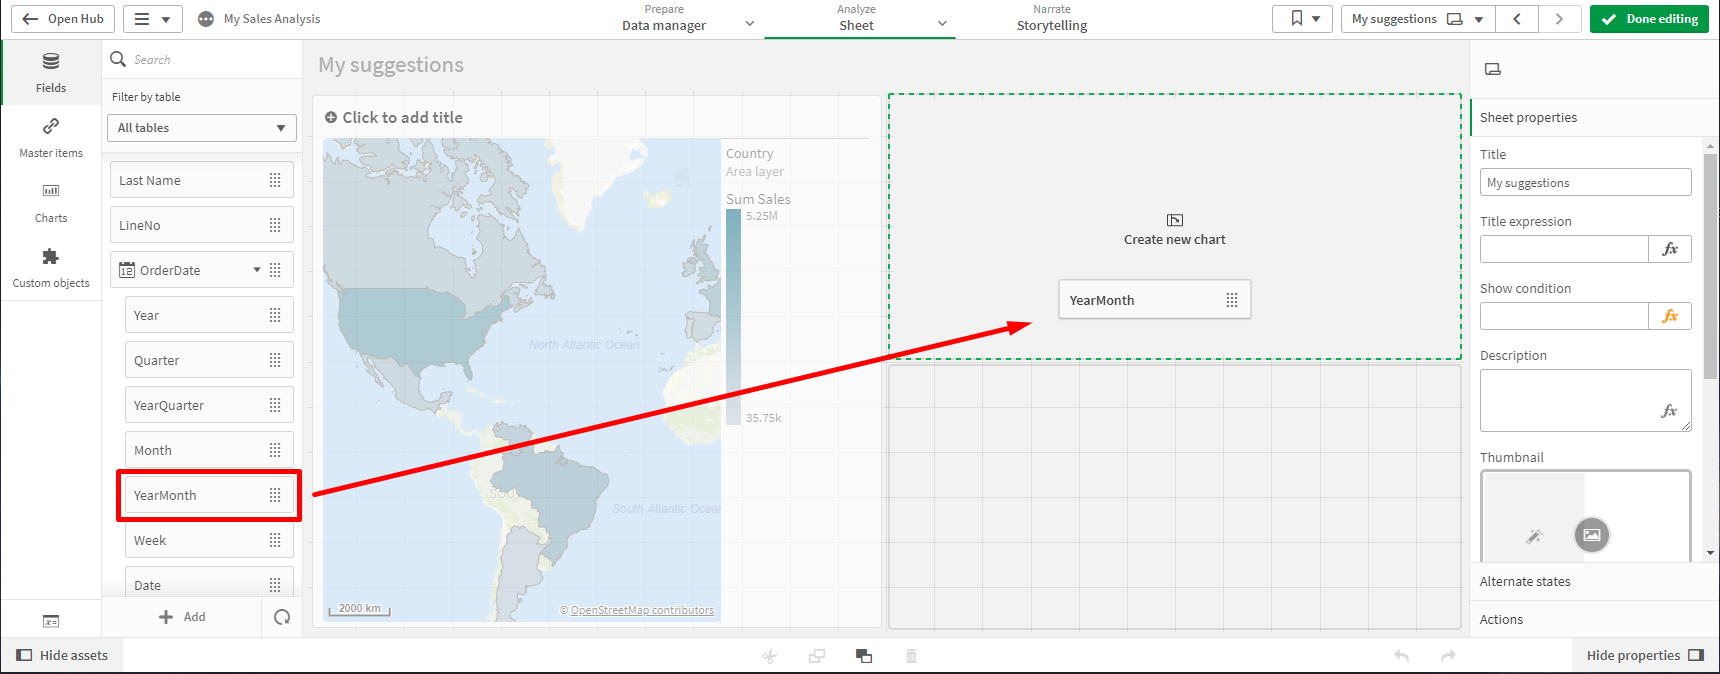
\includegraphics[width=14cm]{./images/19.1} 
	\end{center}

\newpage
\textbf{6.3. Se obtiene un tipo de gráfico de tabla. }

    \begin{center}
		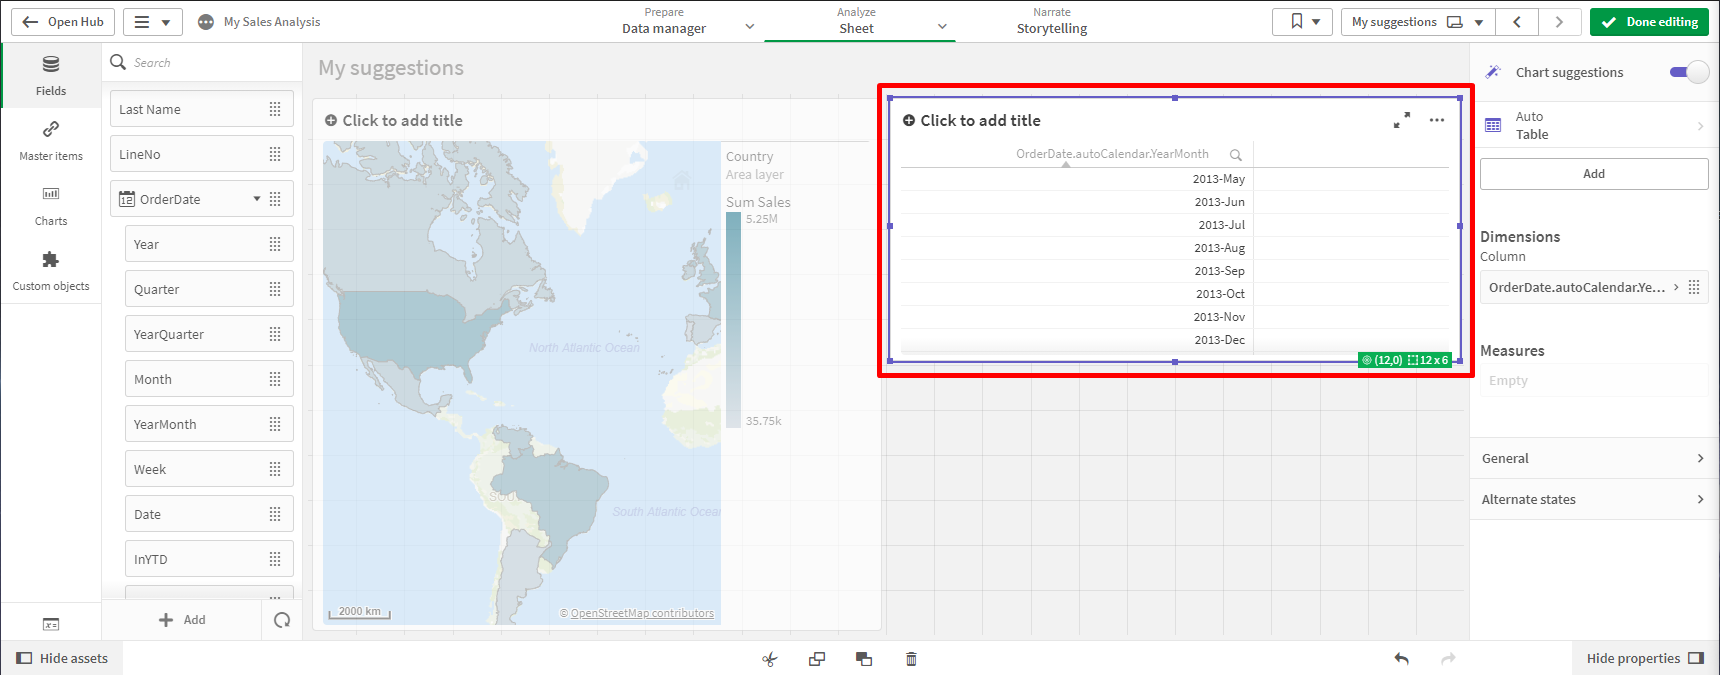
\includegraphics[width=14cm]{./images/19.2} 
	\end{center}

\textbf{6.4. Arrastre y suelte el campo \textit{Sales} para 
cubrir toda la tabla que actualmente muestra los valores de año y 
mes para los pedidos. }

    \begin{center}
		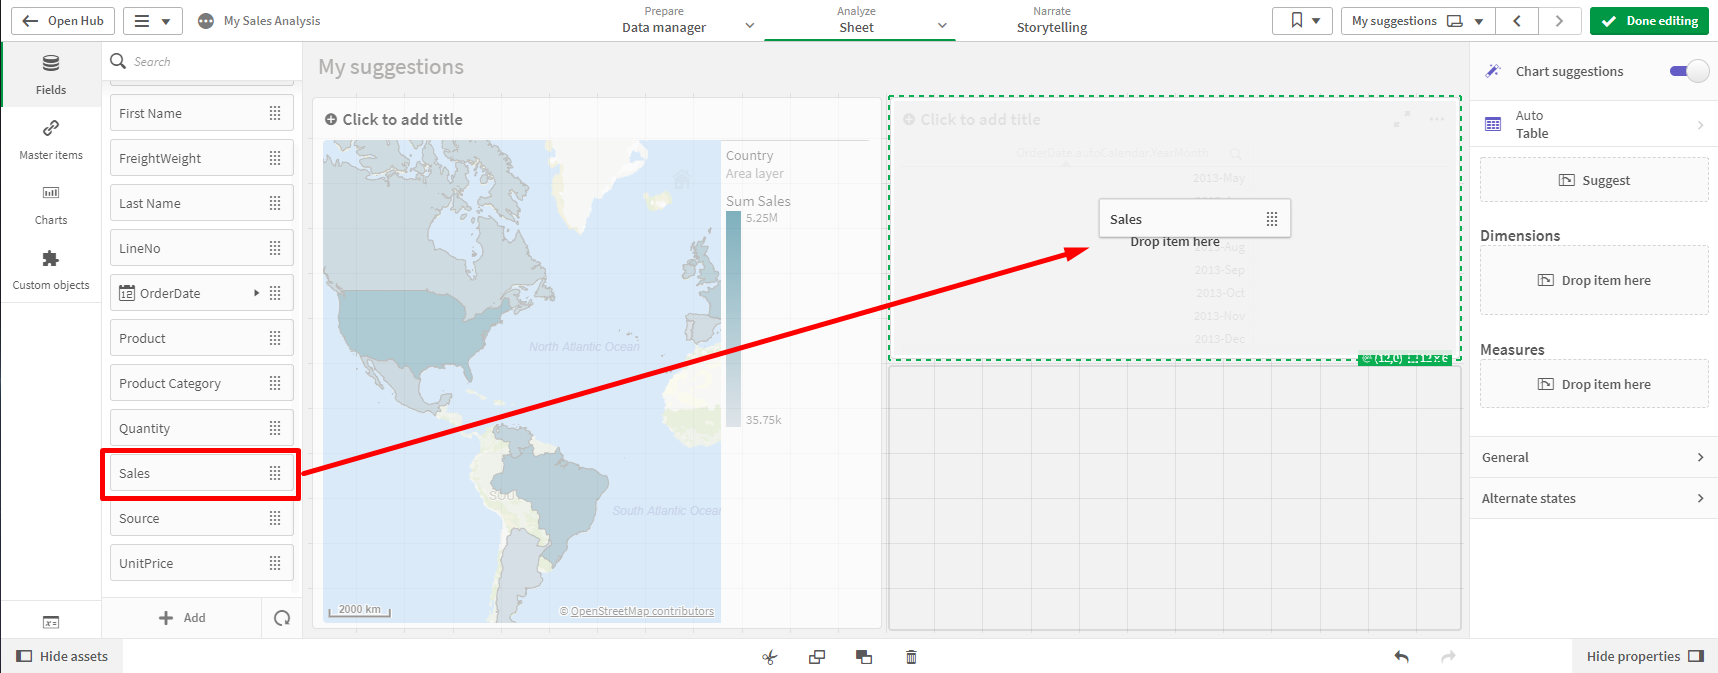
\includegraphics[width=14cm]{./images/20} 
	\end{center}
\newpage
\textbf{6.5. Se obtiene un gráfico de líneas, debido al
 hecho de que se ha proporcionado una dimensión de fecha 
y un campo de valores de medida a esta visualización.}

    \begin{center}
		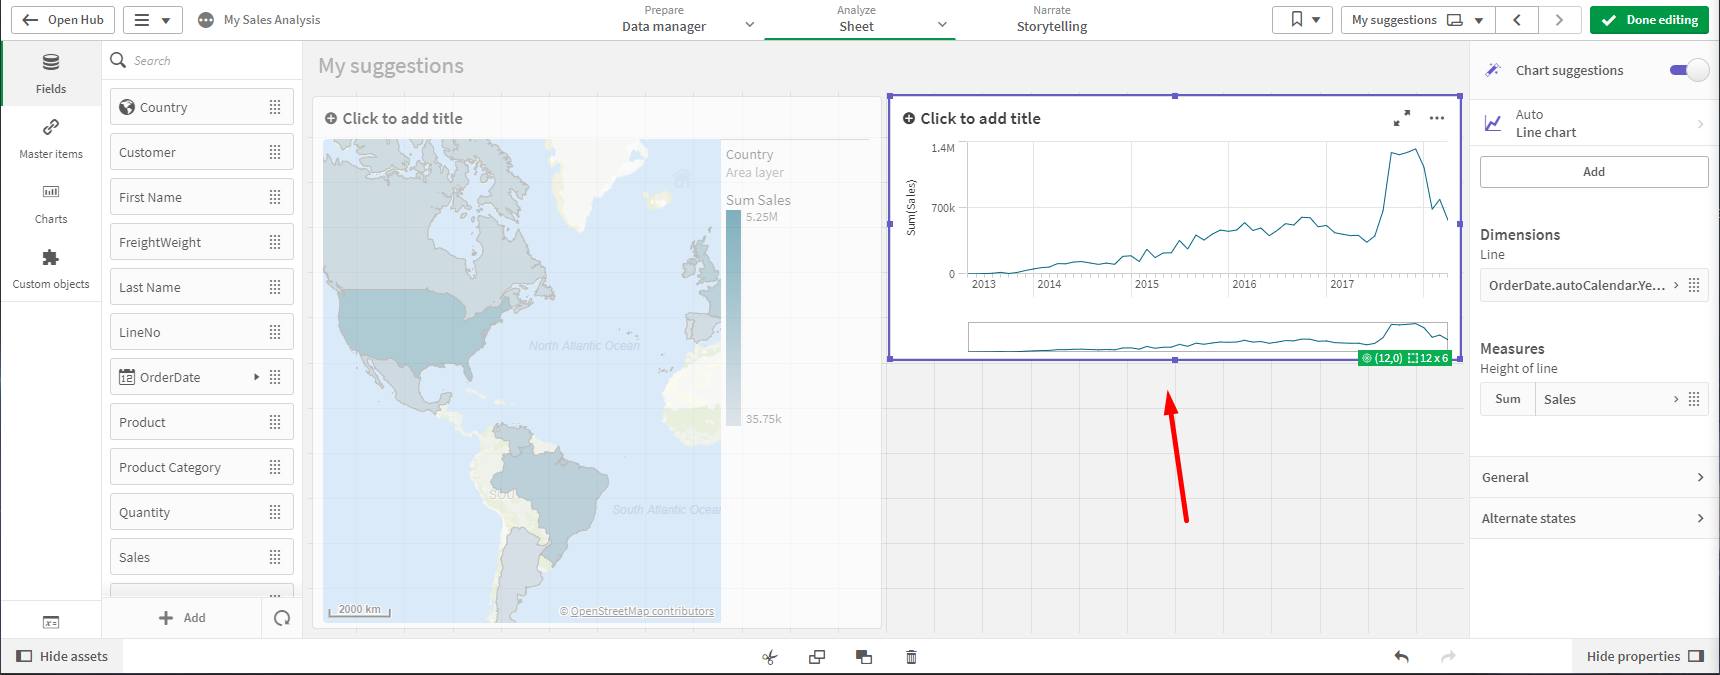
\includegraphics[width=14cm]{./images/21} 
	\end{center}

\textbf{6.6. Arrastre y suelte el campo \textit{Quantity} para 
cubrir todo el gráfico de líneas. }

    \begin{center}
		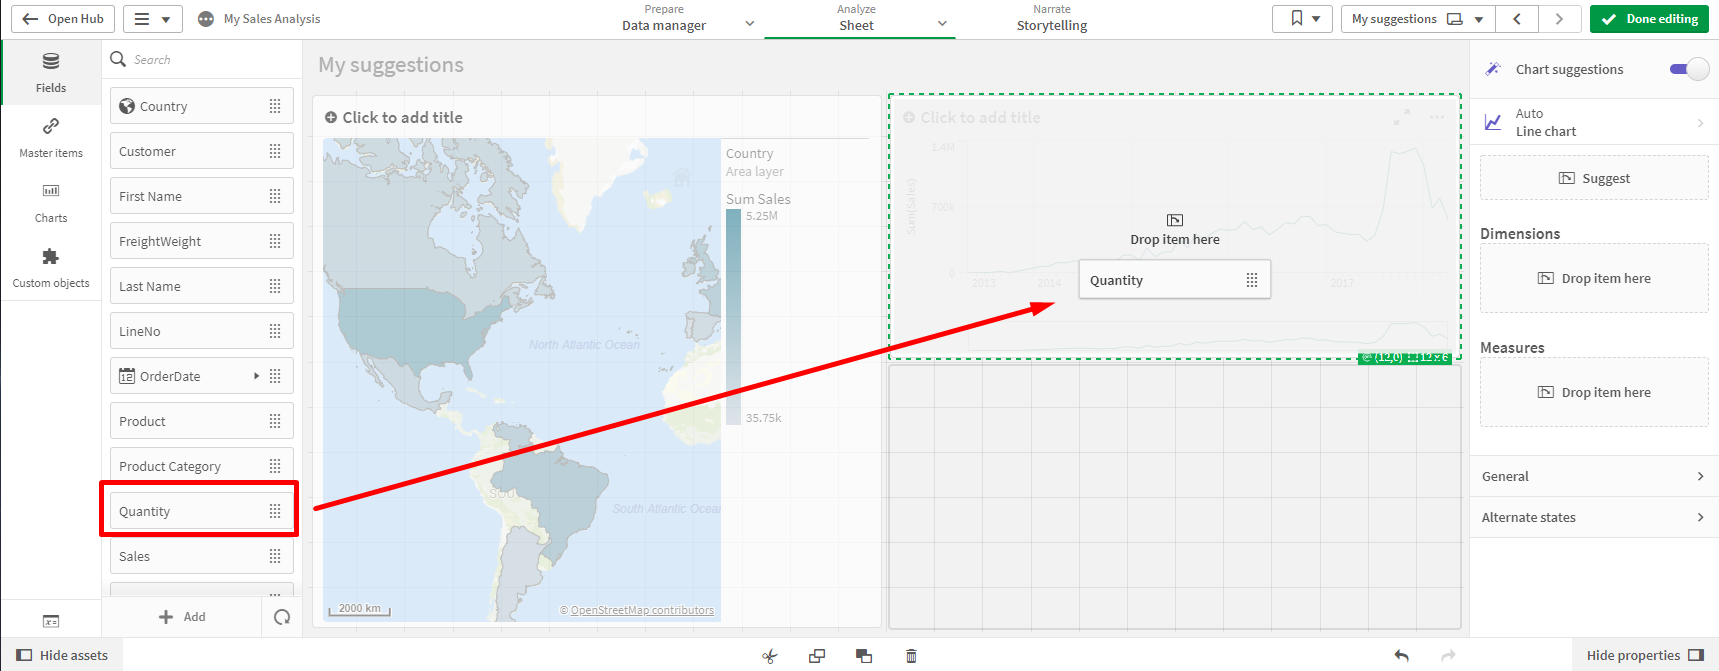
\includegraphics[width=14cm]{./images/22} 
	\end{center}
\newpage
\textbf{6.7. Se obtiene un gráfico combinado, debido al hecho de 
que se proporcionaron una dimensión y múltiples medidas 
(que ocupan diferentes rangos) y haga clic en el botón \textbf{Done editing}..}

    \begin{center}
		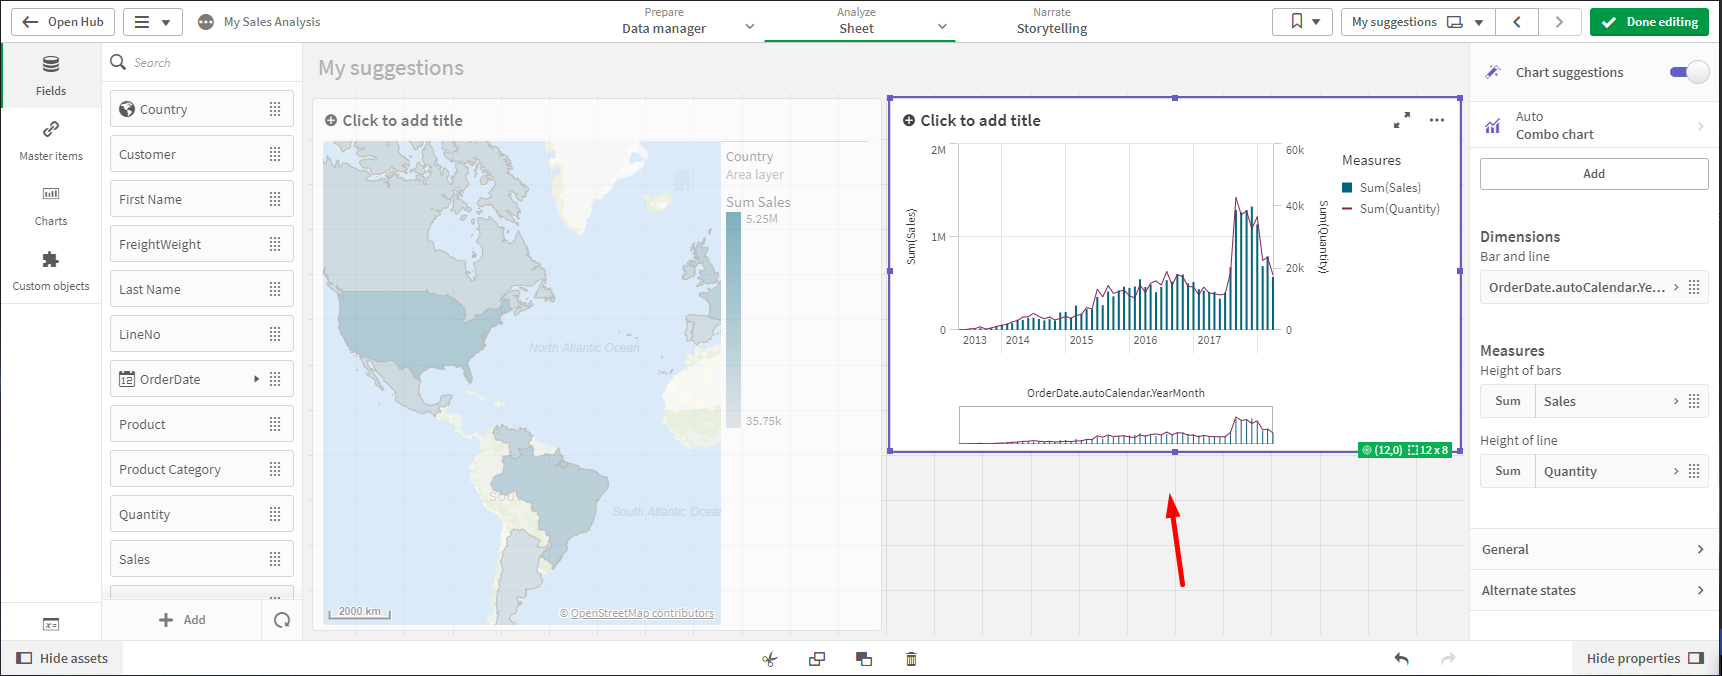
\includegraphics[width=14cm]{./images/22.1} 
	\end{center}
	 \begin{center}
		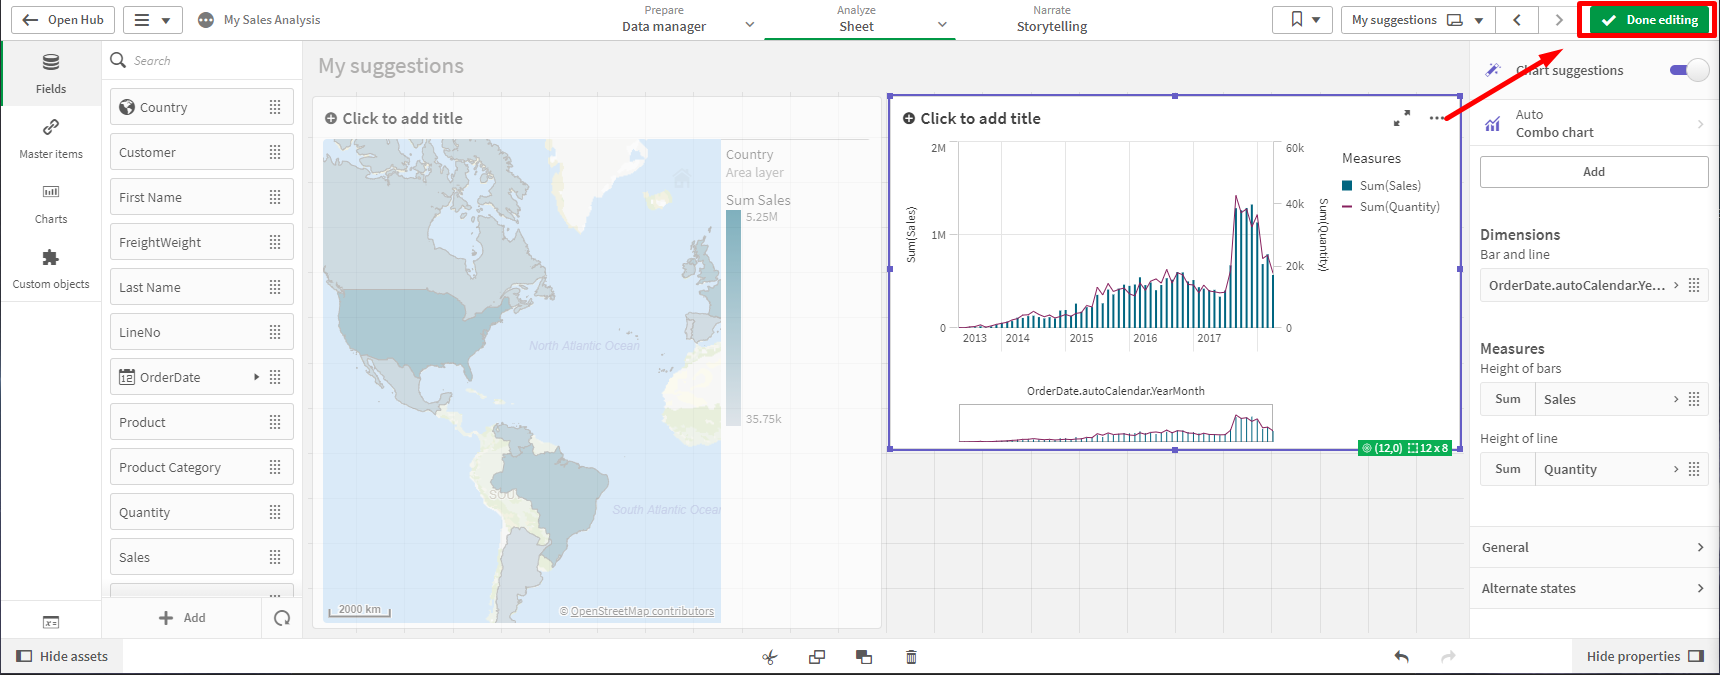
\includegraphics[width=14cm]{./images/22.2} 
	\end{center}
\newpage
\textbf{6.8. Use el control deslizante de zoom del minigráfico,
 debajo del gráfico combinado, para examinar los valores más
 recientes de mes y año.}

    \begin{center}
		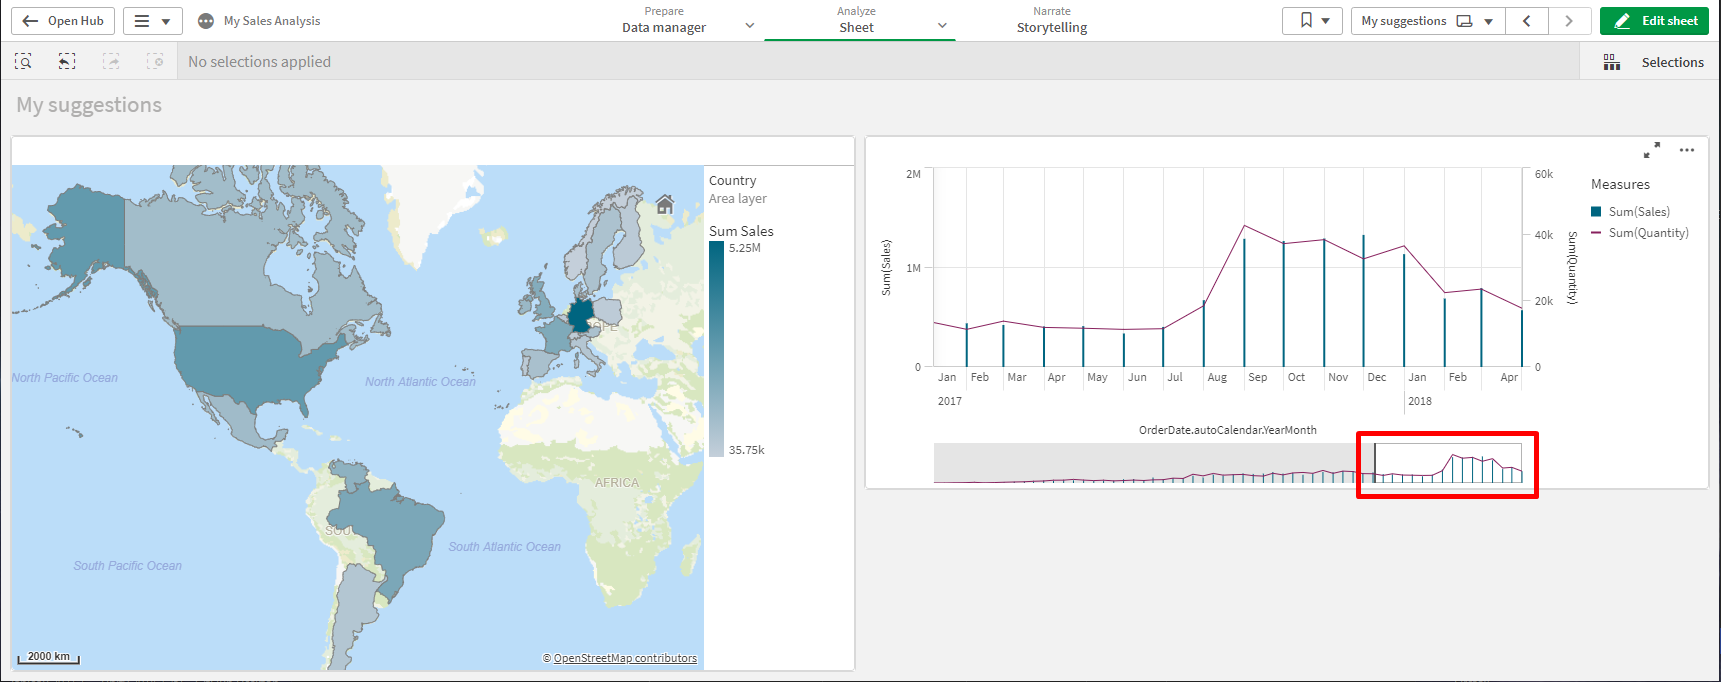
\includegraphics[width=14cm]{./images/22.3} 
	\end{center}

\newpage


\section{Pruebe un tipo de gráfico alternativo sugerido}

\textbf{7.1. Vuelva al modo \textbf{Editar hoja} y considere 
sugerencias de gráficos alternativos.}

    \begin{center}
		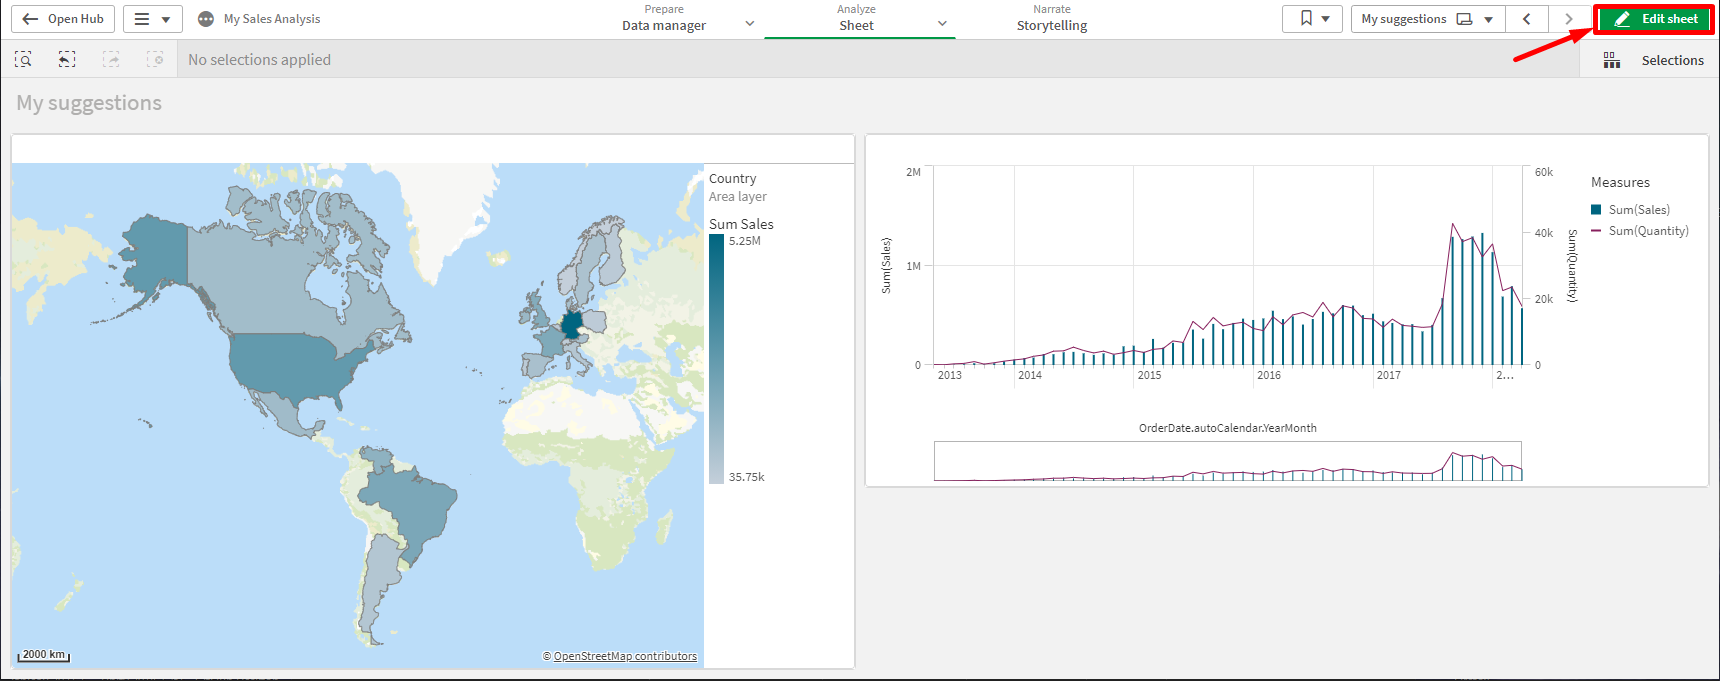
\includegraphics[width=14cm]{./images/23} 
	\end{center}

\textbf{7.2. Cambie del gráfico \textbf{Combo chart} a 
un \textbf{Line chart}.}

    \begin{center}
		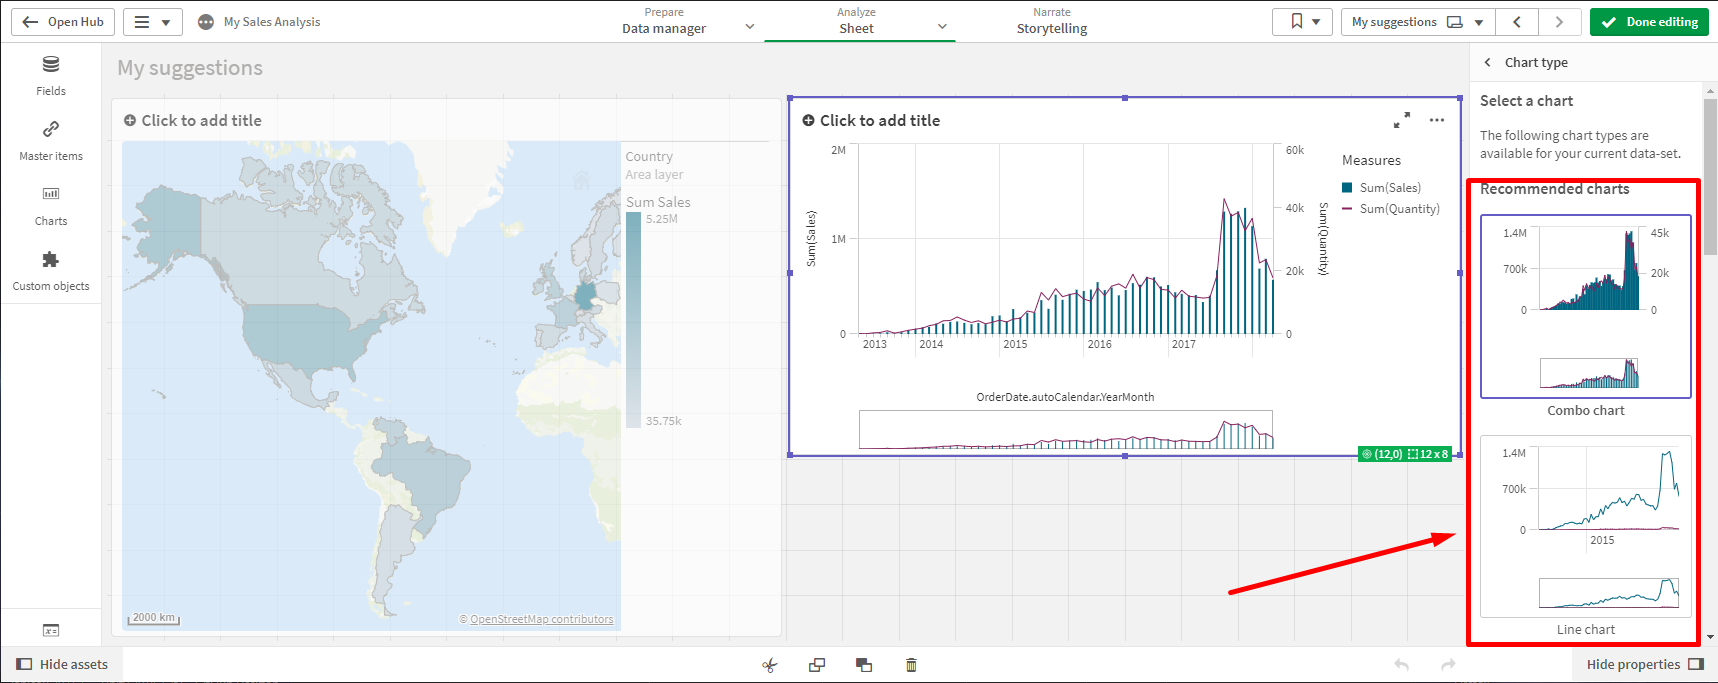
\includegraphics[width=14cm]{./images/23.1} 
	\end{center}
	\newpage

	
\newpage	
\section{Cambie el interruptor de sugerencias de 
gráficos de ‘on’ a ‘off’}

\textbf{8.1. Nos gustaría ajustar la combinación de colores 
aplicada a las formas de los países en el gráfico de mapa, así
 que cambie el interruptor de \textbf{Chart suggestions} a \textbf{‘off’}.}

    \begin{center}
		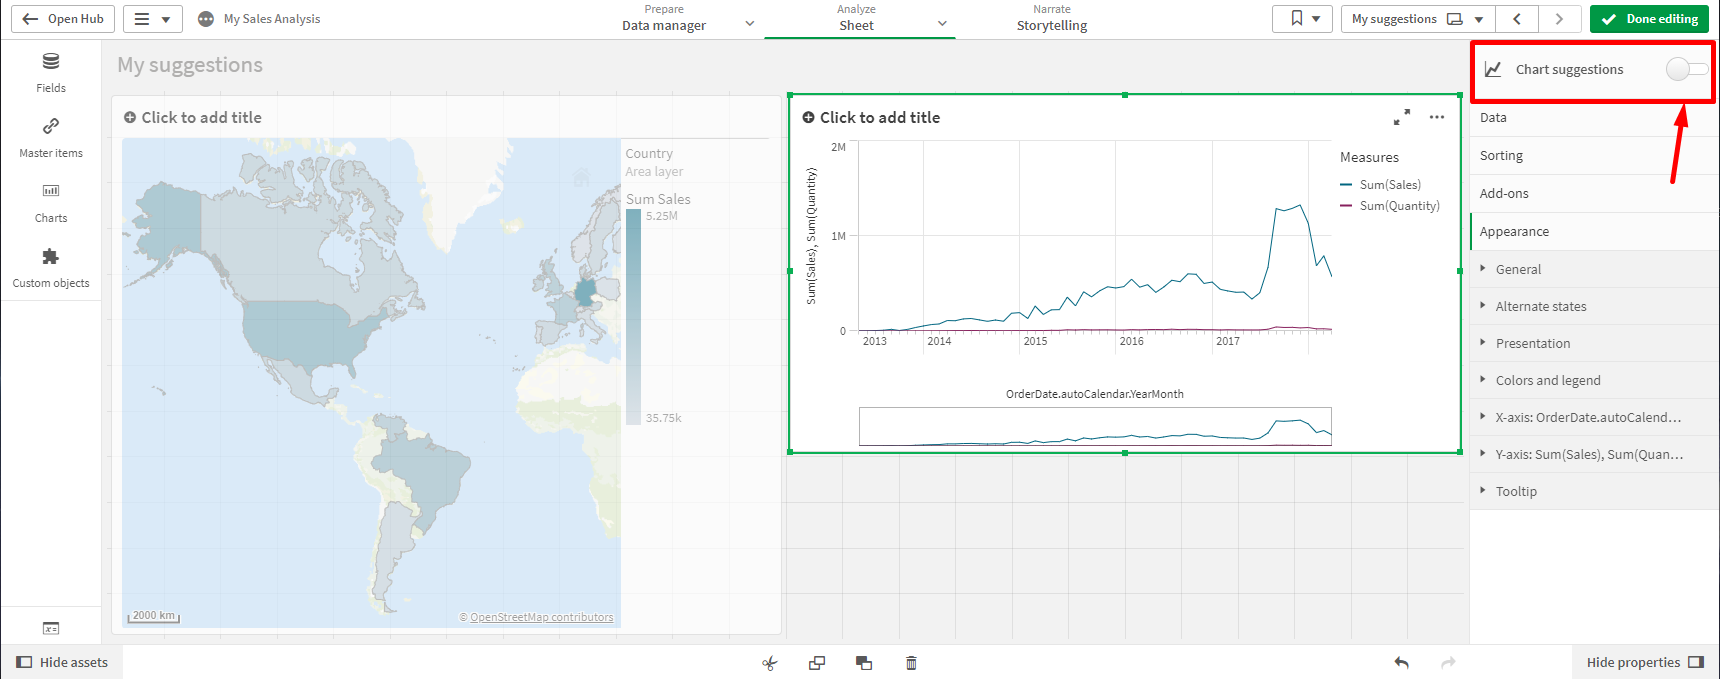
\includegraphics[width=14cm]{./images/24} 
	\end{center}
	
\textbf{8.2. HAbra la sección \textbf{Layers} del panel de
 propiedades y haga clic en \textit{Area Layer} de \textbf{Country}.}

    \begin{center}
		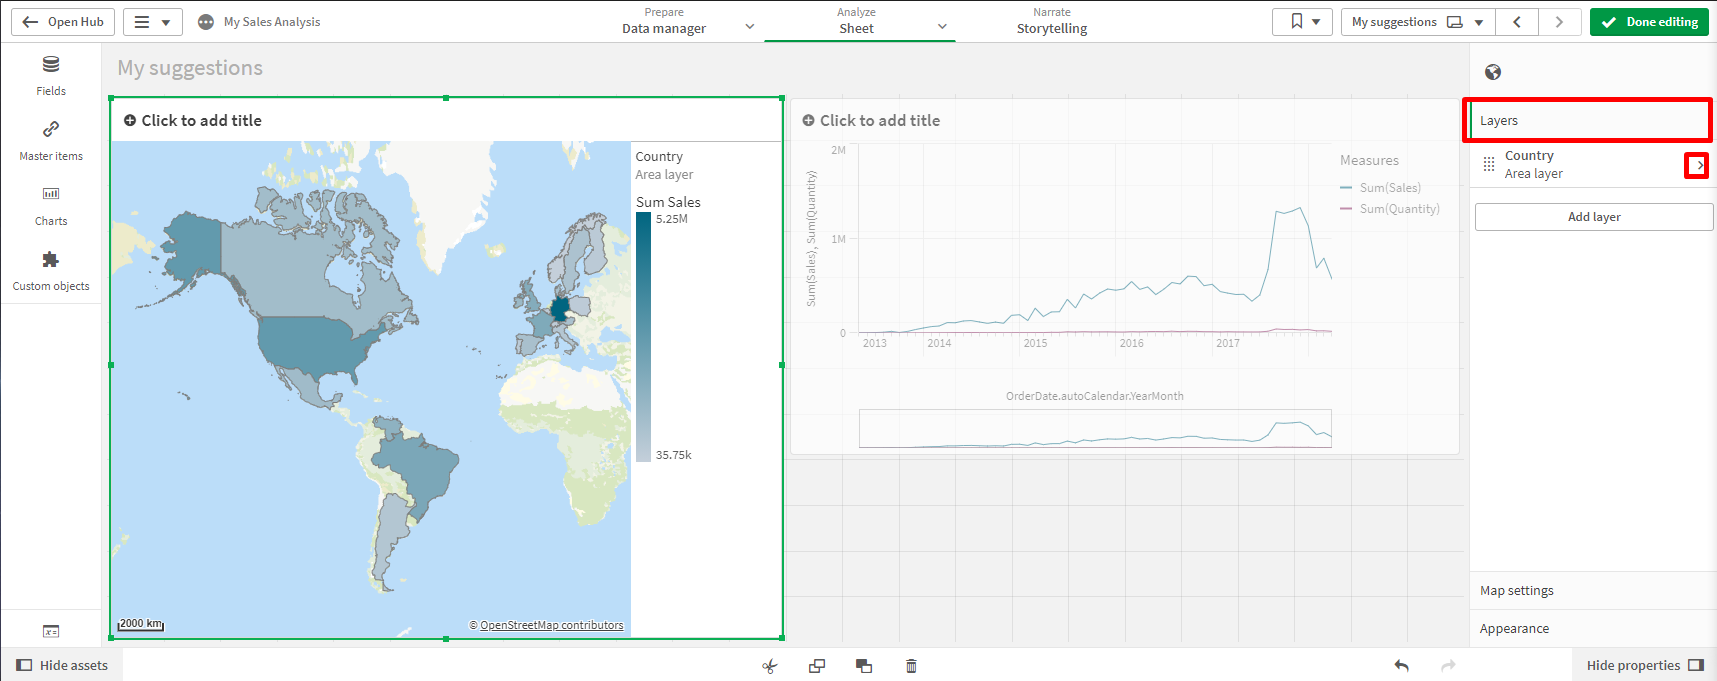
\includegraphics[width=14cm]{./images/25} 
	\end{center}
\newpage	
\textbf{8.3. Abra la sección \textbf{Colors} y busque 
la opcion \textbf{Color scheme}.}

    \begin{center}
		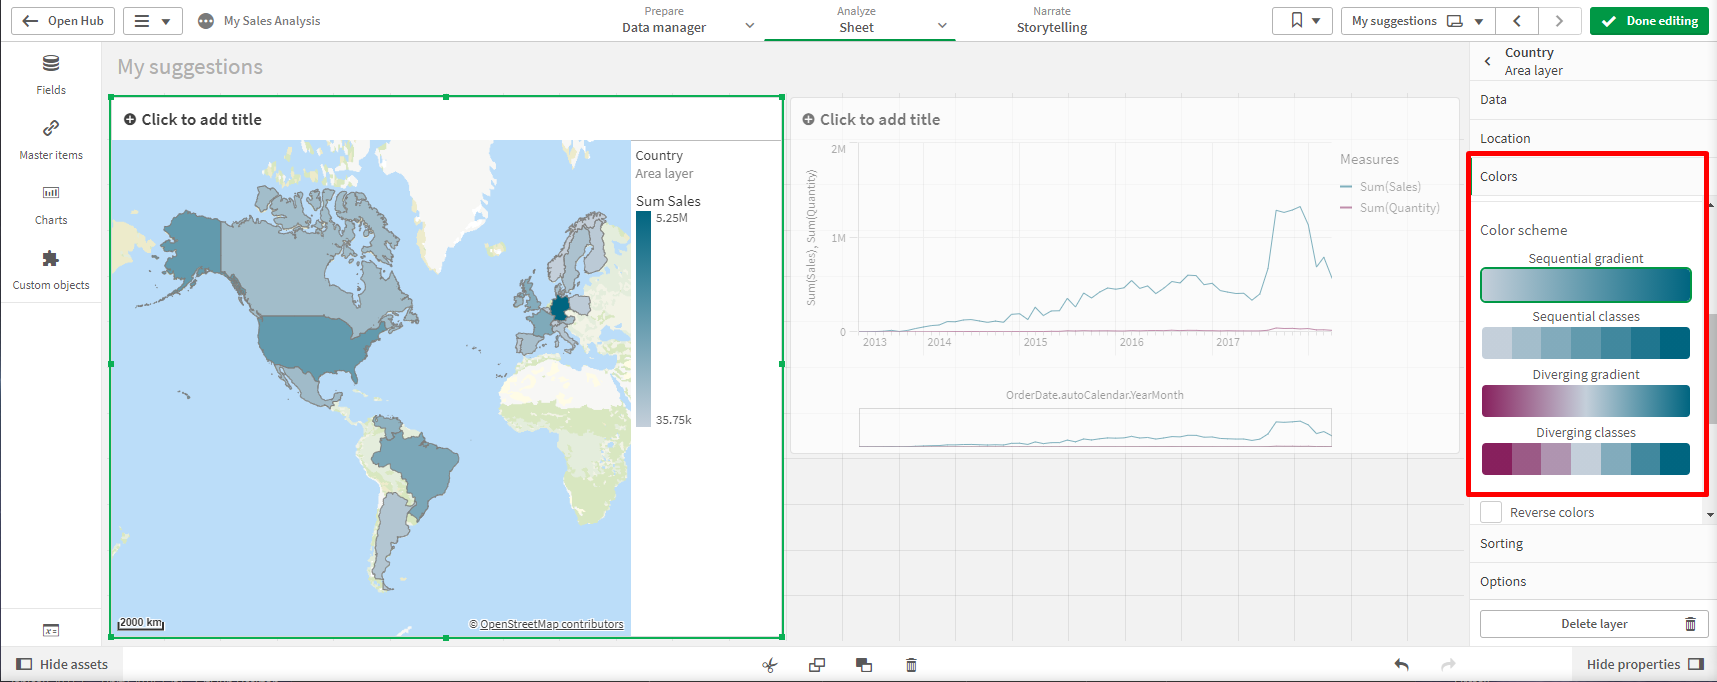
\includegraphics[width=14cm]{./images/26} 
	\end{center}
	
\textbf{8.4. Cambie el esquema de 
color de \textbf{Sequential gradient} a \textbf{Diverging gradient}.}

    \begin{center}
		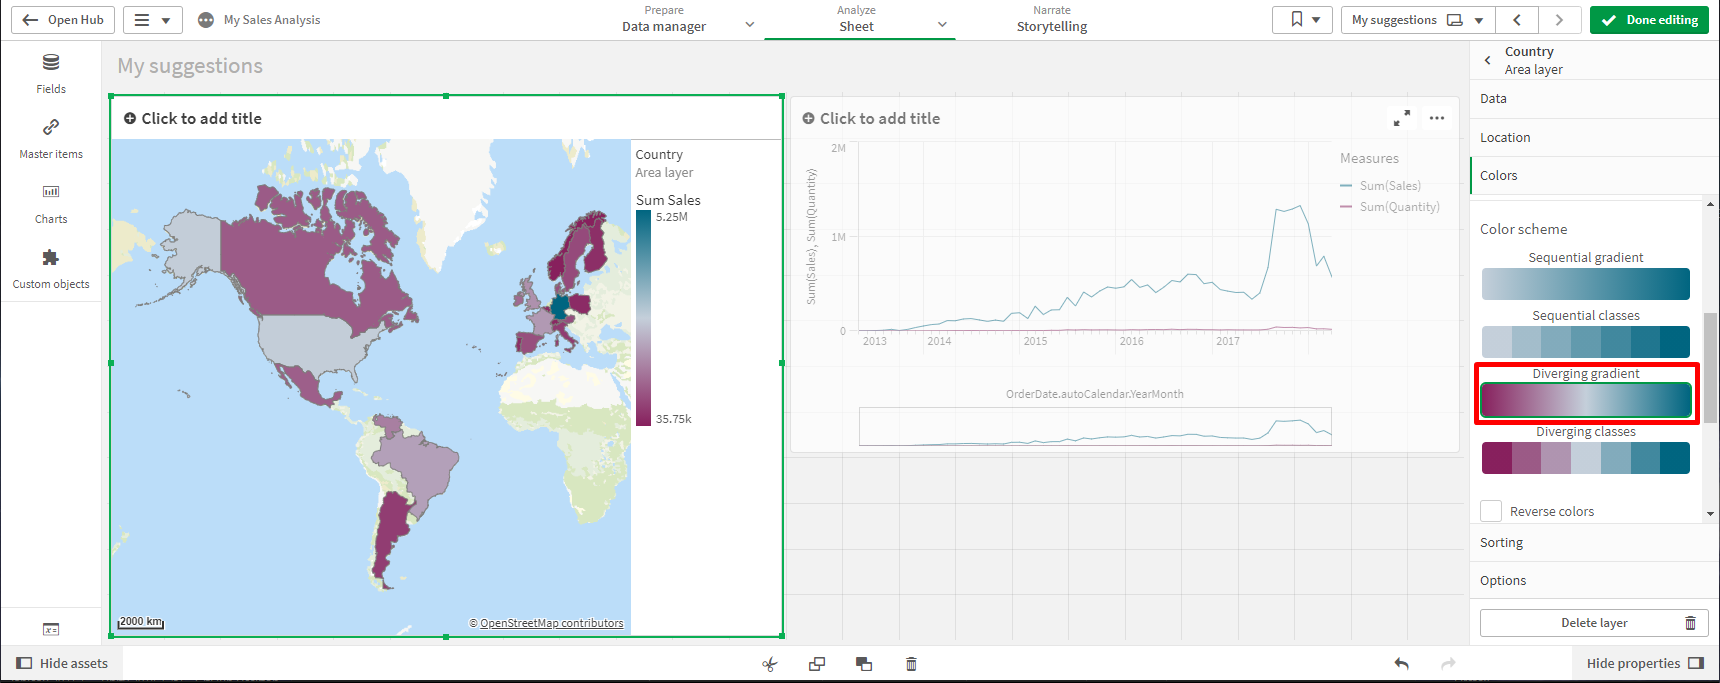
\includegraphics[width=14cm]{./images/26.1} 
	\end{center}
\newpage	
\textbf{8.5. Marque la casilla de 
verificación \textbf{Reverse colors}.}

    \begin{center}
		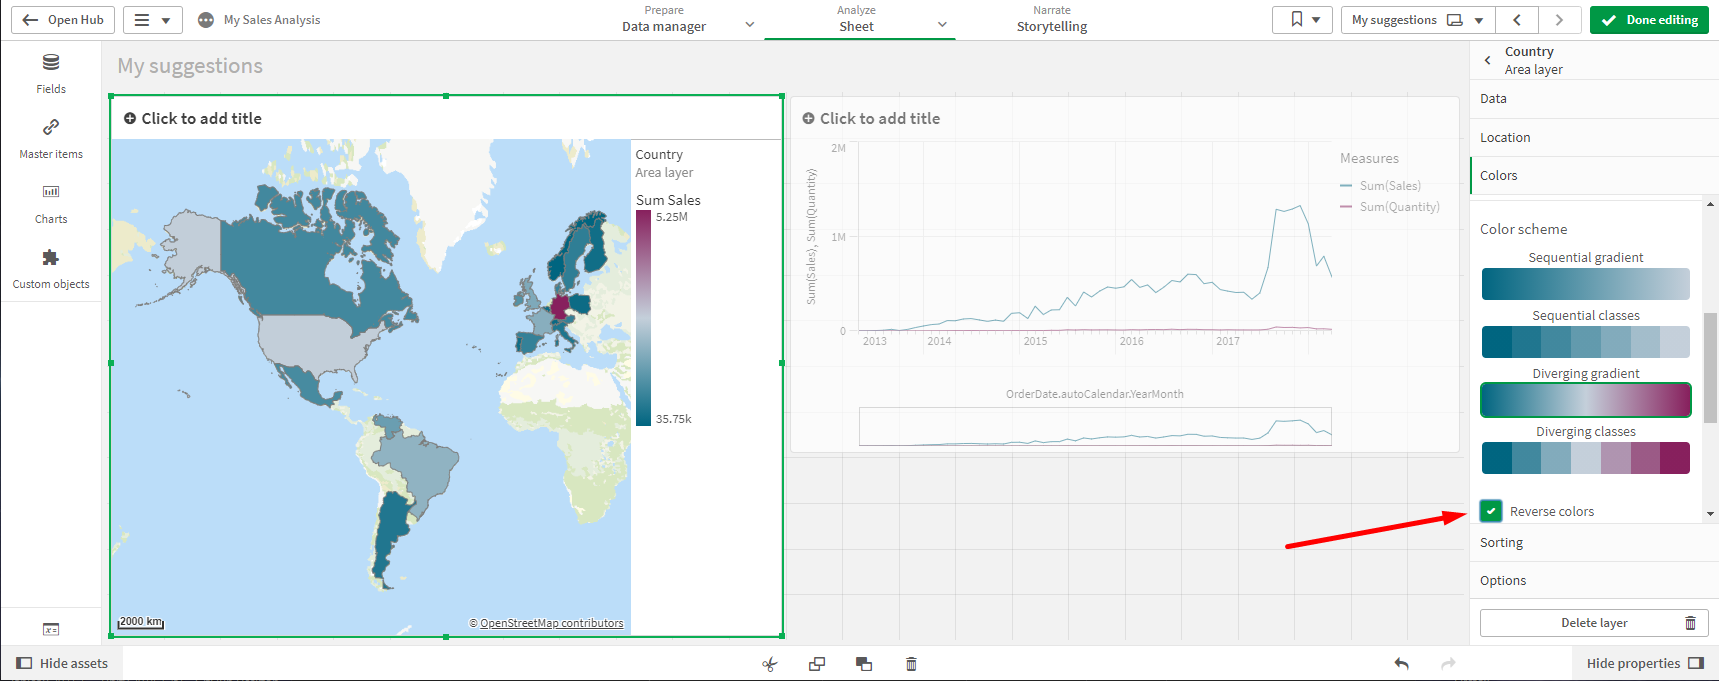
\includegraphics[width=14cm]{./images/26.2} 
	\end{center}
	
\textbf{8.6. El mapa resultante debería aparecer 
como se ve a continuación.}

    \begin{center}
		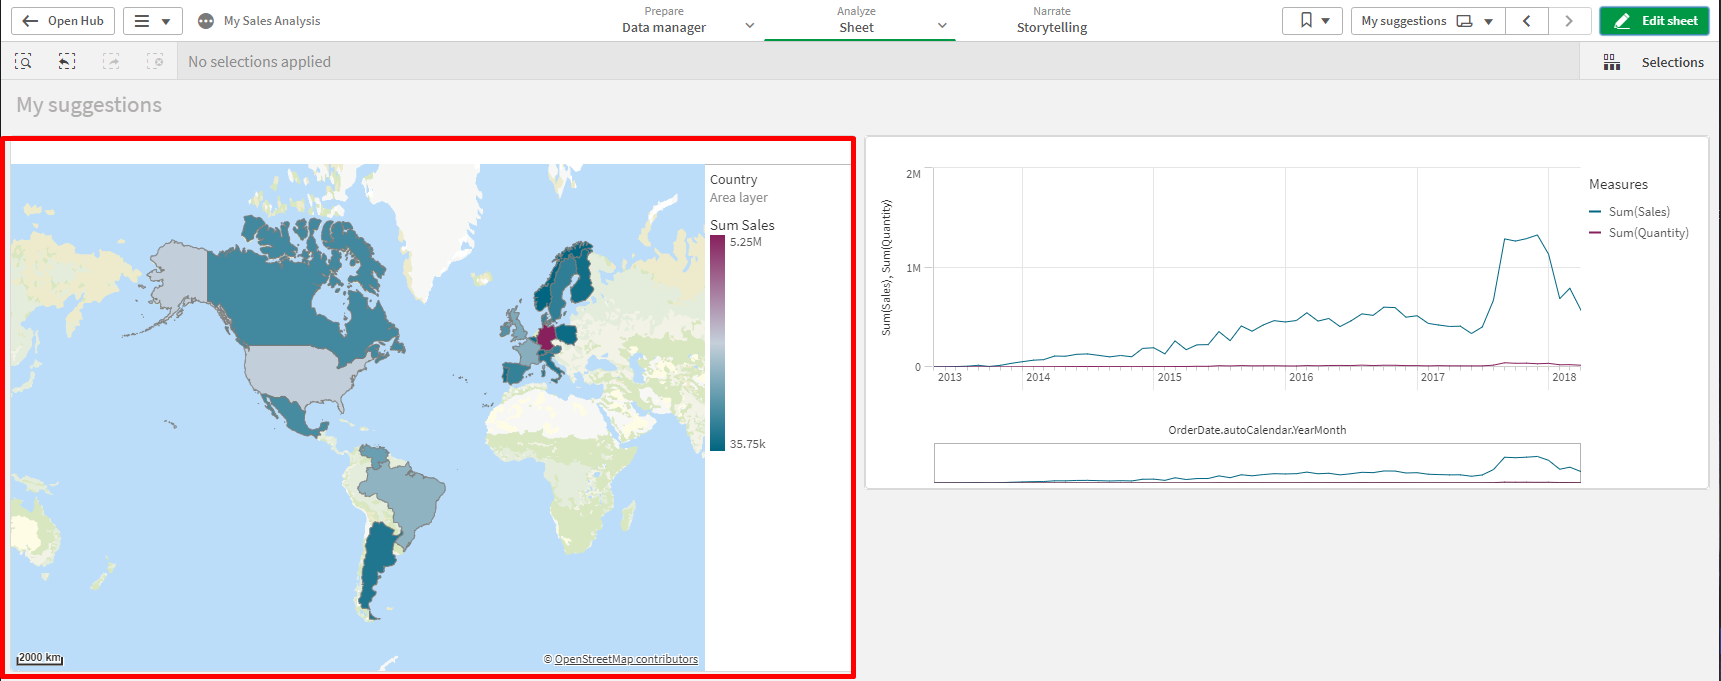
\includegraphics[width=14cm]{./images/27} 
	\end{center}

\newpage
\end{document}